% - - - - - - - - - - SUBSECTION - - - - - - - - - - %
\subsection{The fundamentals of access control}

% * * * * * * NEW FRAME * * * * * * %
\begin{frame}{Glossary of access control: use case}
    \begin{center}
        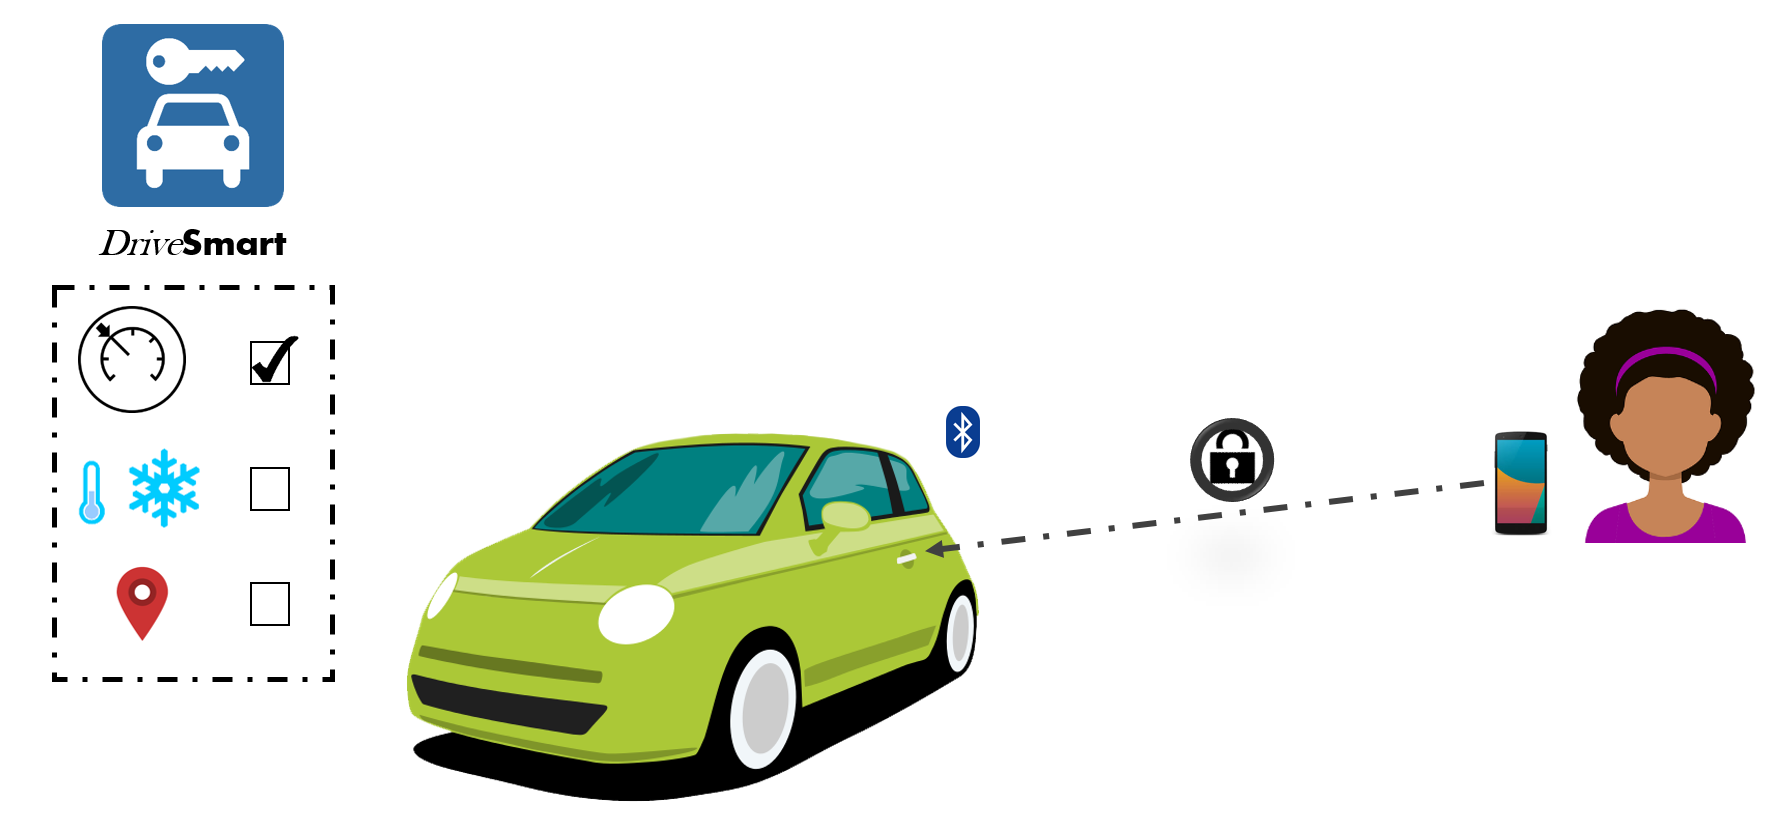
\includegraphics[scale=0.33]{Figures/ex_intro_1.png}
    \end{center}
\end{frame}

% * * * * * * NEW FRAME * * * * * * %
\begin{frame}{Glossary of access control: objects}
    \begin{center}
        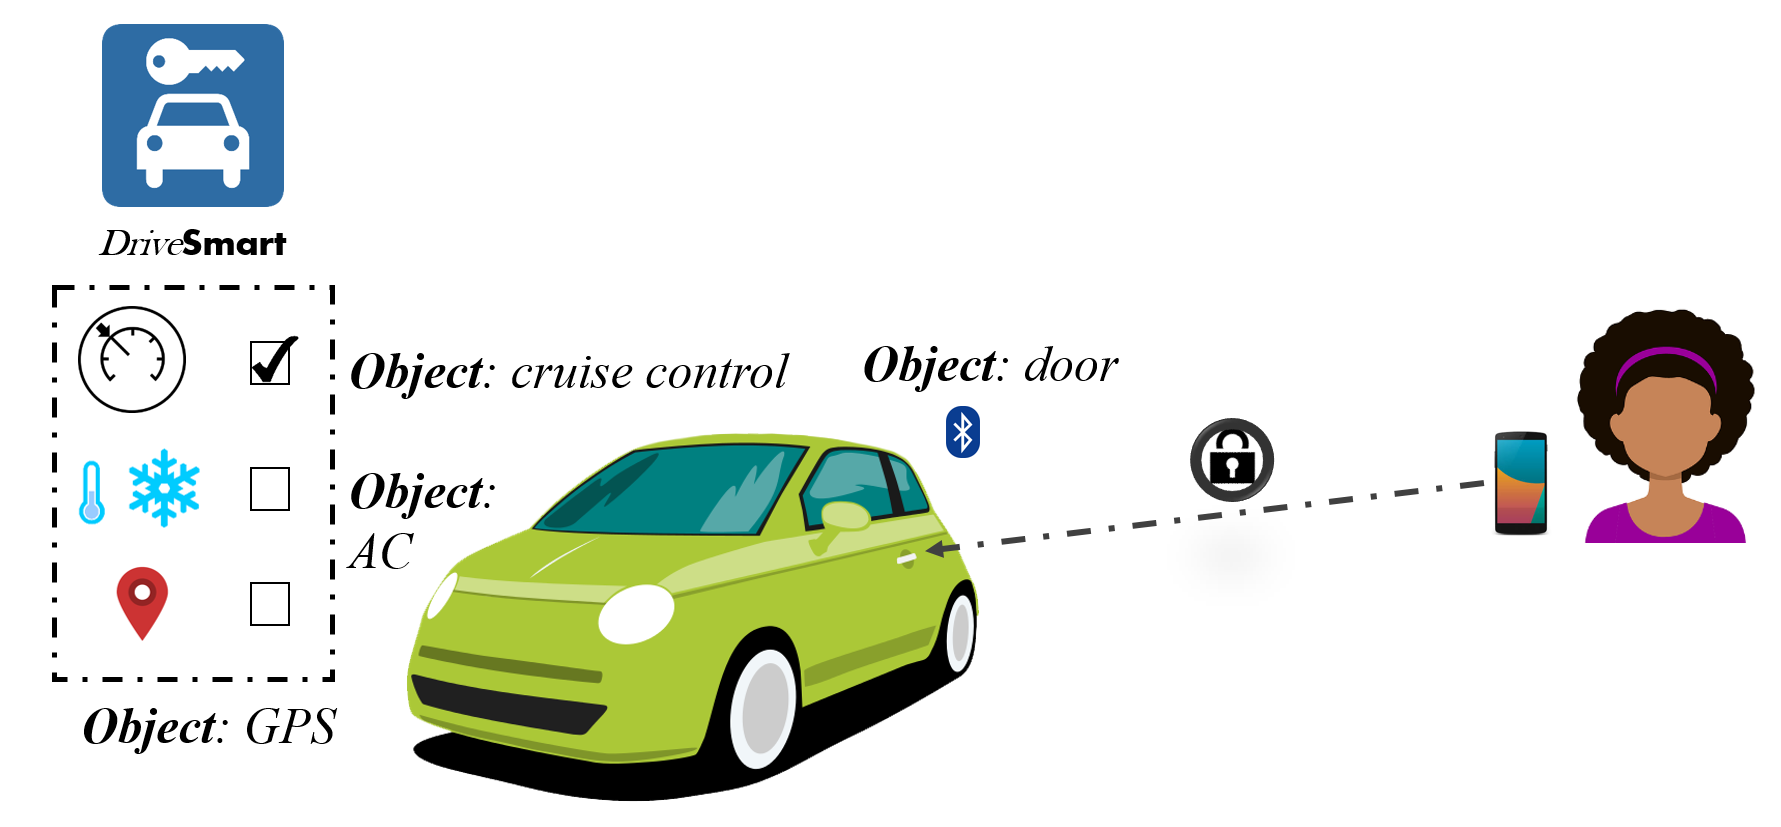
\includegraphics[scale=0.33]{Figures/ex_intro_2.png}
    \end{center}
    
    \begin{definition}
        The \alert{object} is what is to be accessed. 
            \newline \emph{Ex: the cruise control of a smart car, its AC, the doors, etc}
    \end{definition}
\end{frame}

% * * * * * * NEW FRAME * * * * * * %
\begin{frame}{Glossary of access control: subjects}
    \begin{center}
        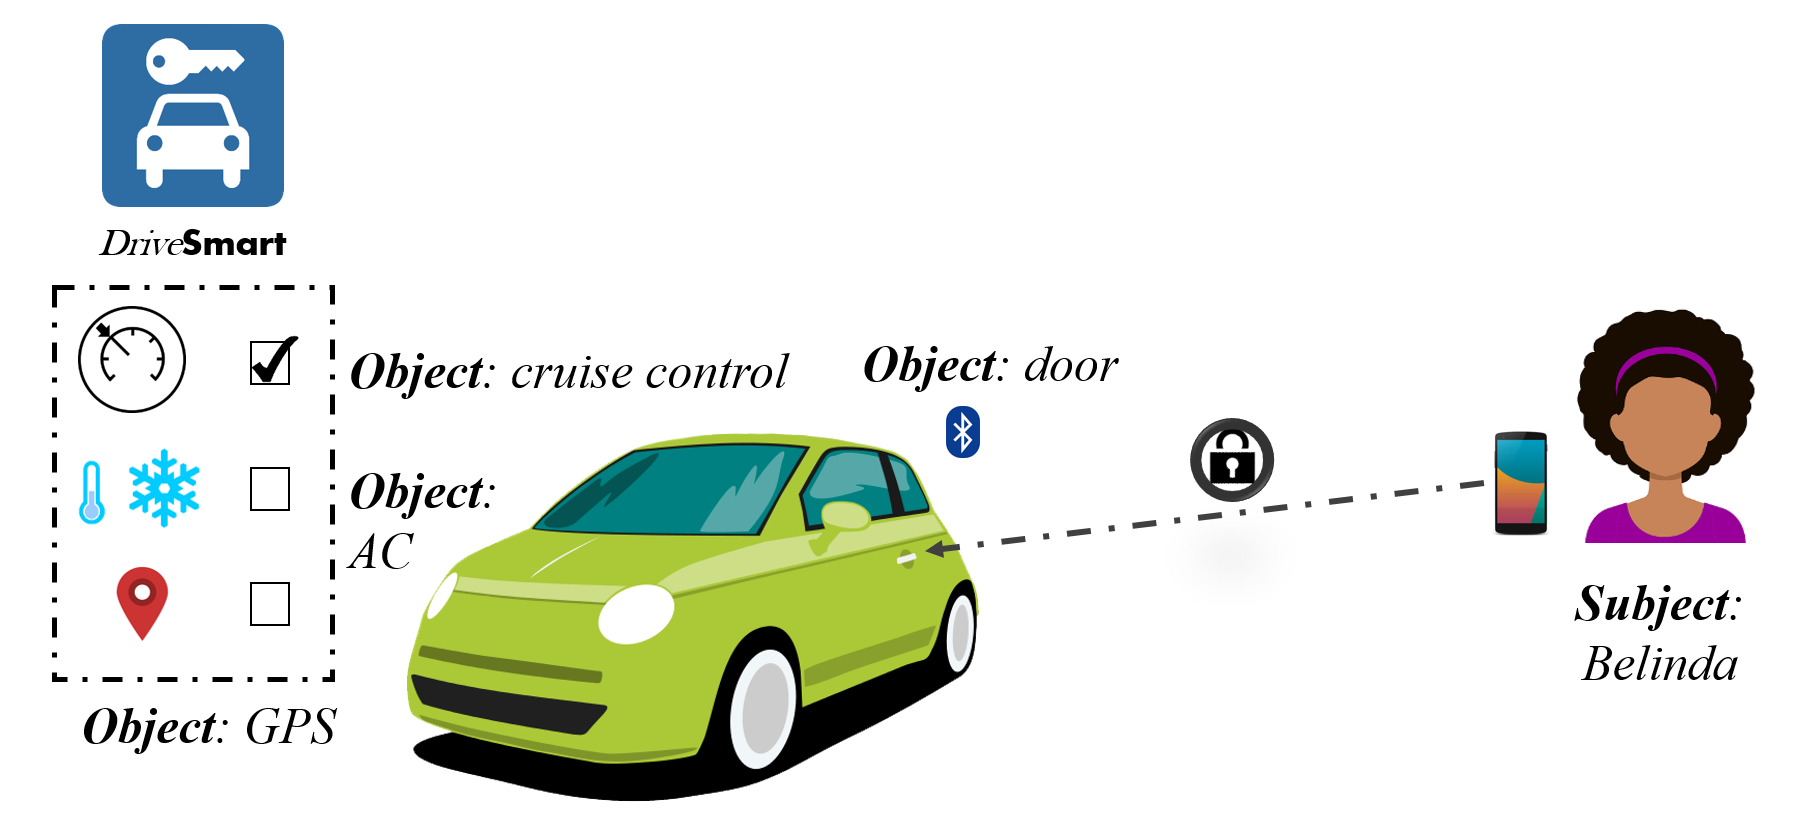
\includegraphics[scale=0.33]{Figures/ex_intro_3.png}
    \end{center}
    
    \begin{definition}
        The \alert{subject} is the entity that wishes to access the object.
            \newline \emph{Ex: the driver of the smart car, the owner, passengers}
    \end{definition}
\end{frame}

% * * * * * * NEW FRAME * * * * * * %
\begin{frame}{Glossary of access control: operations}
    \begin{center}
        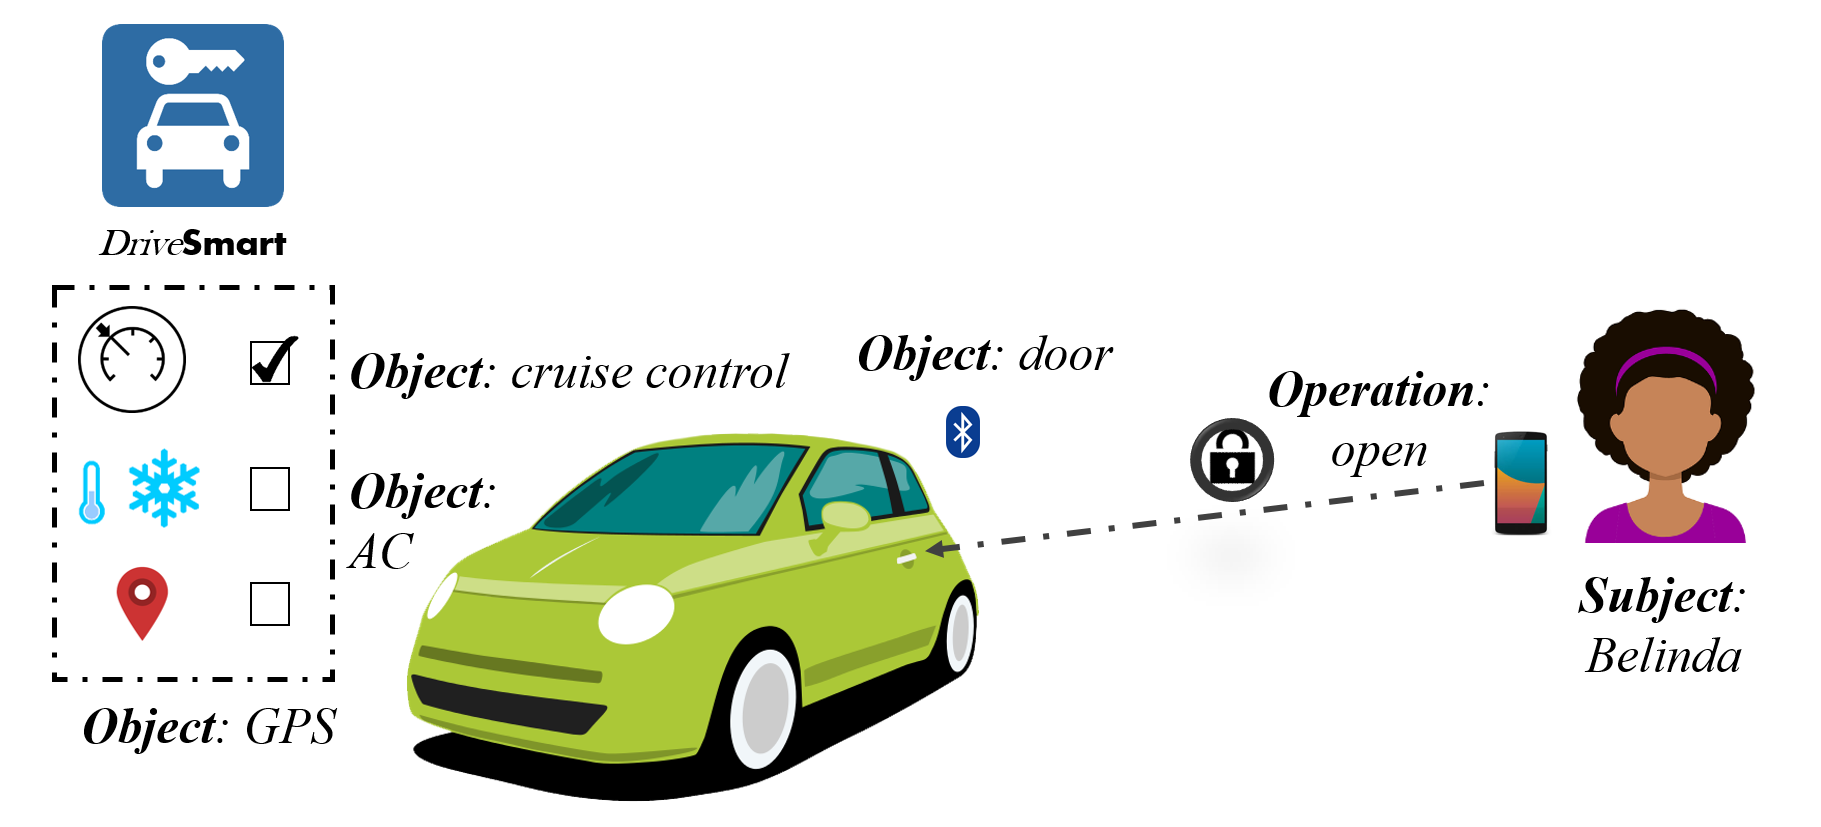
\includegraphics[scale=0.33]{Figures/ex_intro_4.png}
    \end{center}
    
    \begin{definition}
        \alert{Operations} (or actions) are what can be done to a object.
        \newline \emph{Ex: setting the maximum speed, turning on the AC, opening the doors}
    \end{definition}
\end{frame}

% * * * * * * NEW FRAME * * * * * * %
\begin{frame}{Glossary of access control: authorizations}
    \begin{center}
        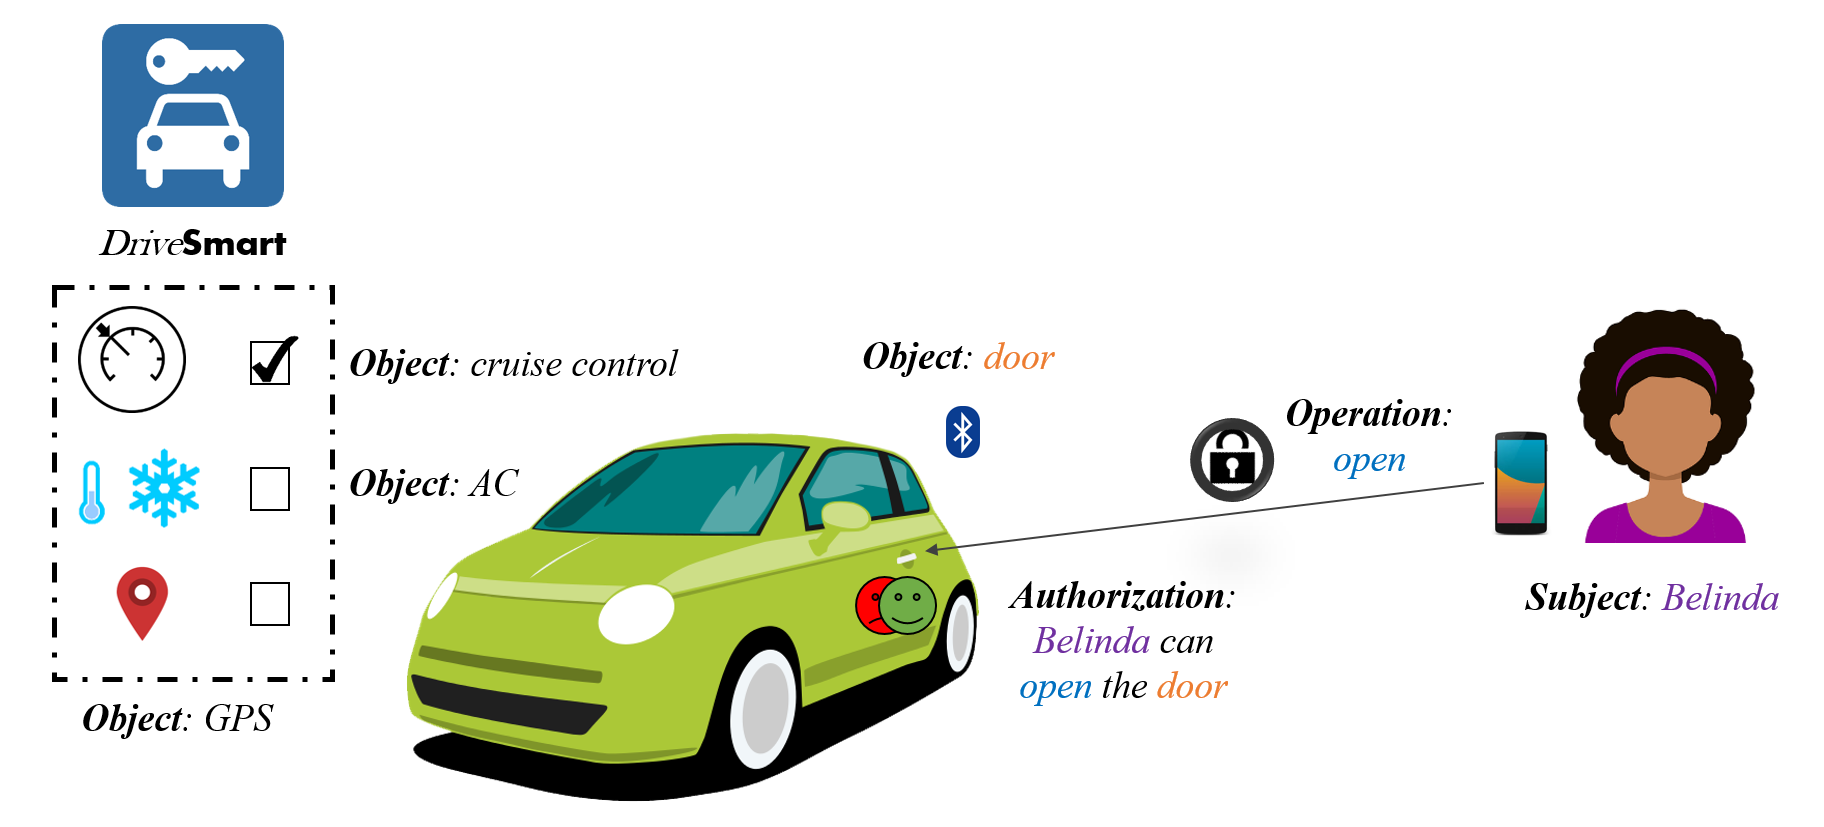
\includegraphics[scale=0.33]{Figures/ex_intro_5.png}
    \end{center}
    
    \begin{definition}
        An \alert{authorization} (or permission/privilege) is the approval granting a subject the right to perform a set of operations on an object.
        \newline \emph{Ex: the owner is allowed to know the location of the car}
    \end{definition}
\end{frame}

% * * * * * * NEW FRAME * * * * * * %
\begin{frame}{Glossary of access control: security domains}
    \begin{center}
        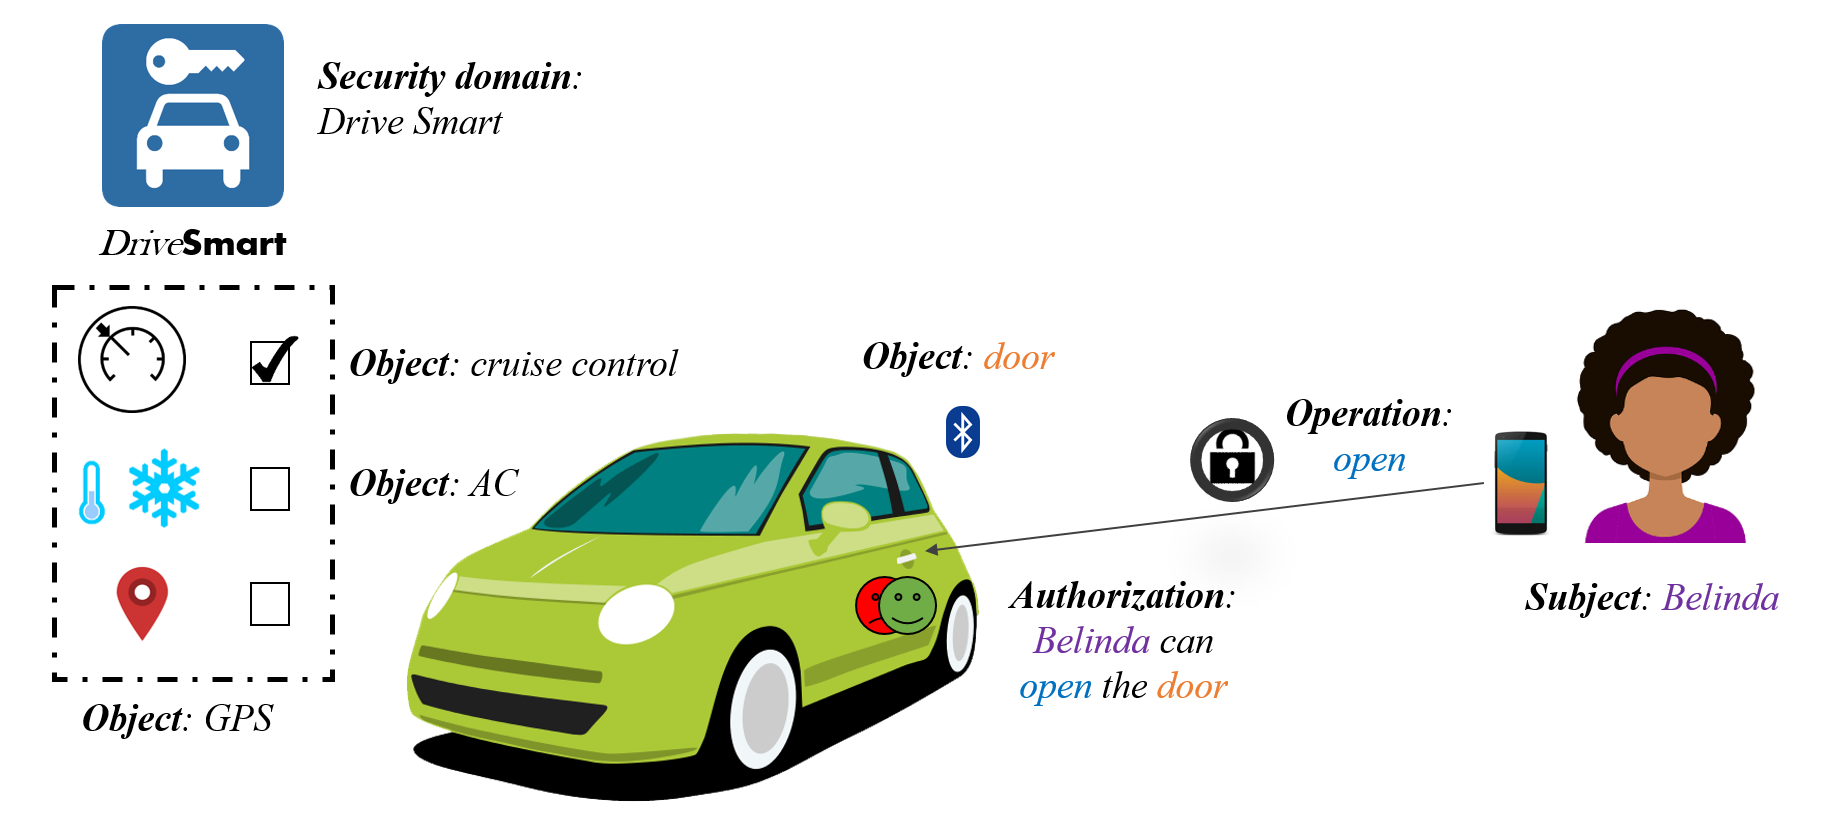
\includegraphics[scale=0.33]{Figures/ex_intro_6.png}
    \end{center}
    
    \begin{definition}
        A \alert{security domain} is an environment with a set of objects, subjects, and security policies.
        \newline \emph{Ex: different car rental companies}
    \end{definition}
\end{frame}

% * * * * * * NEW FRAME * * * * * * %
\begin{frame}{The building blocks of access control}
    \only<1>{
        \begin{center}
            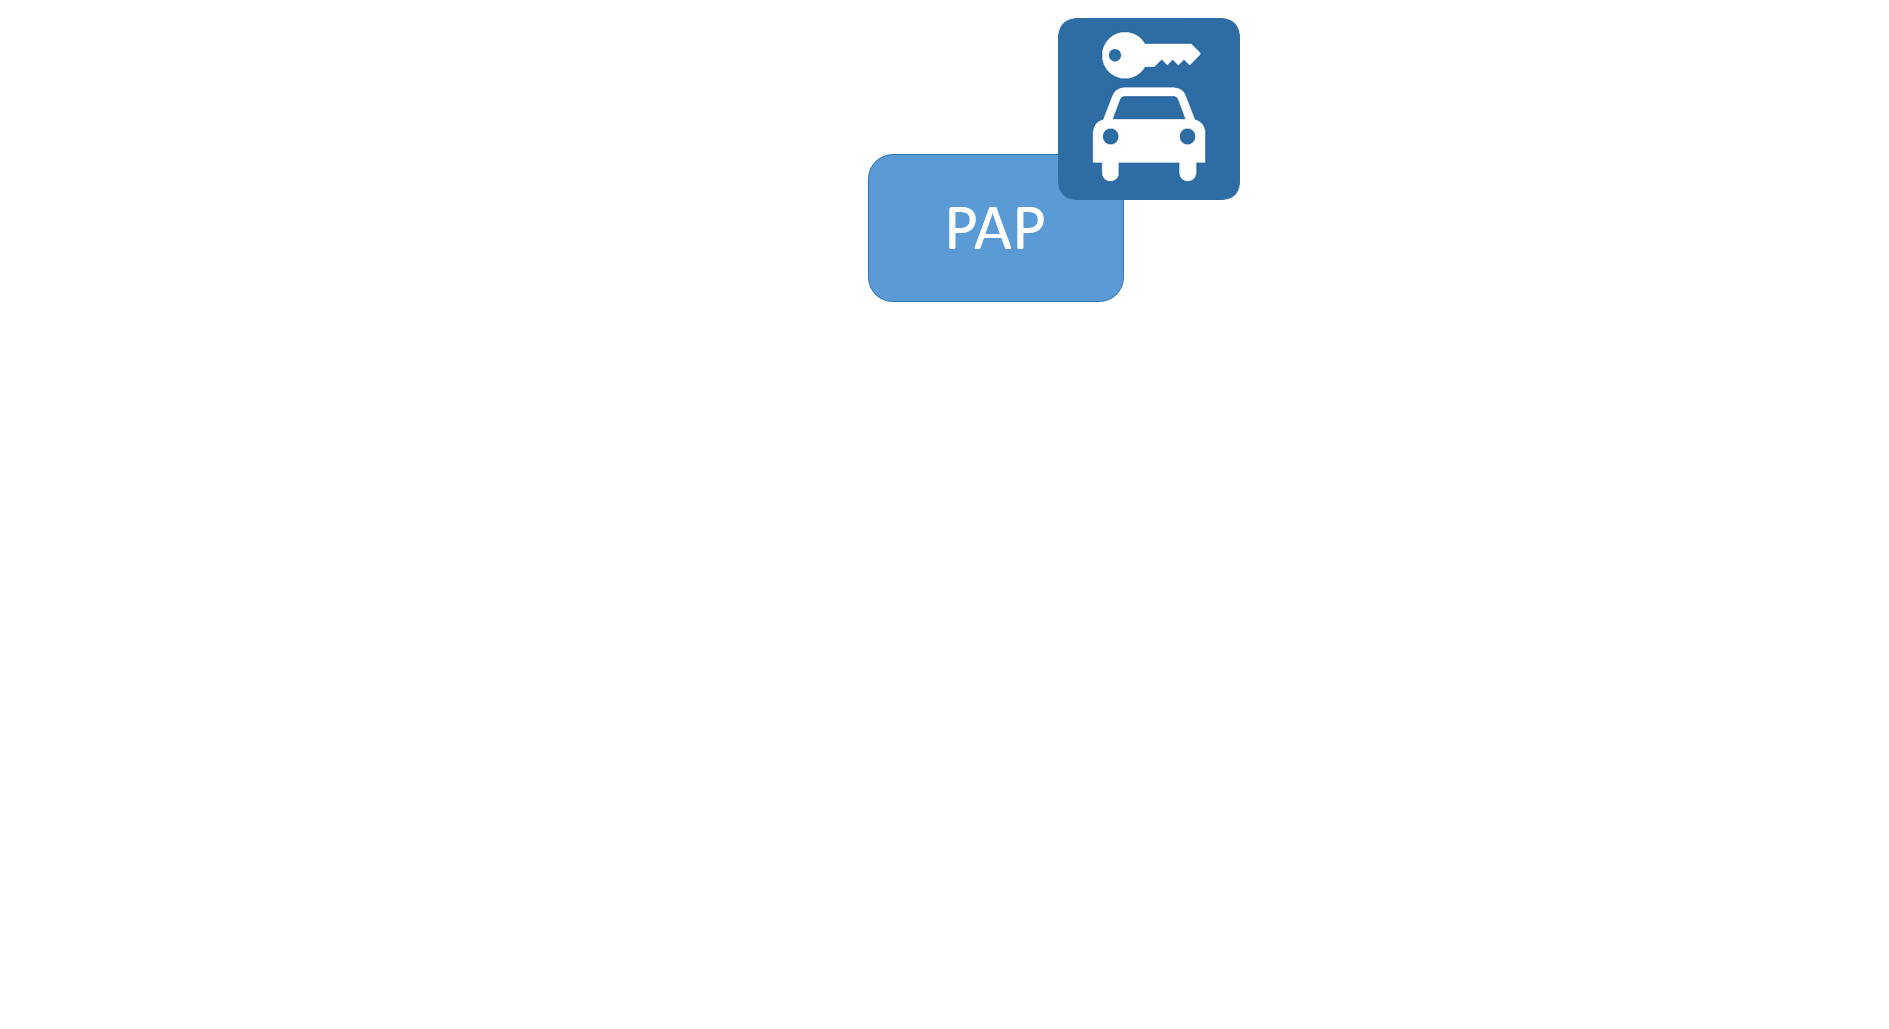
\includegraphics[scale=0.35]{Figures/AC_instance_0.png}
        \end{center}
        
        The \alert{PAP (Policy Administration Point~\cite{RFC3198})} creates the access policies.
    }
        
    \only<2>{
        \begin{center}
            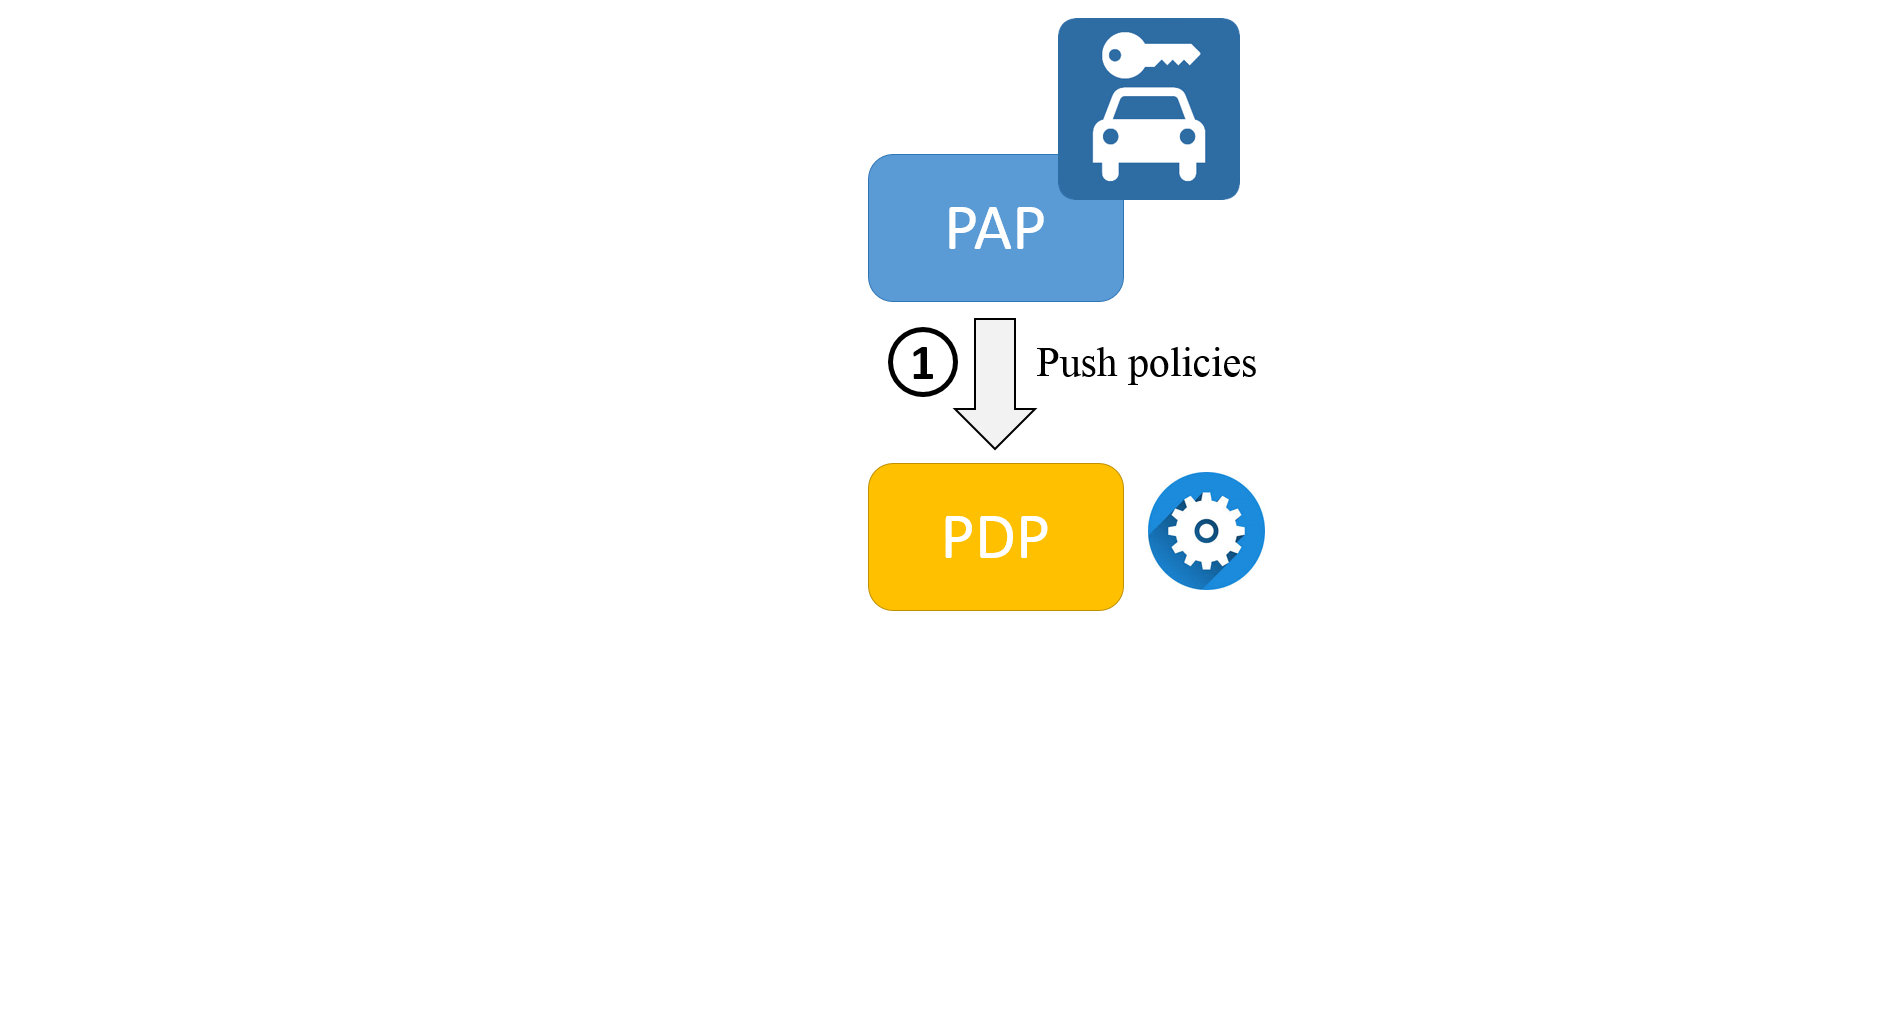
\includegraphics[scale=0.35]{Figures/AC_instance_1.png}
        \end{center}
        
        The \alert{PAP (Policy Administration Point~\cite{RFC3198})} creates the access policies.
        }
        
    \only<3>{
        \begin{center}
            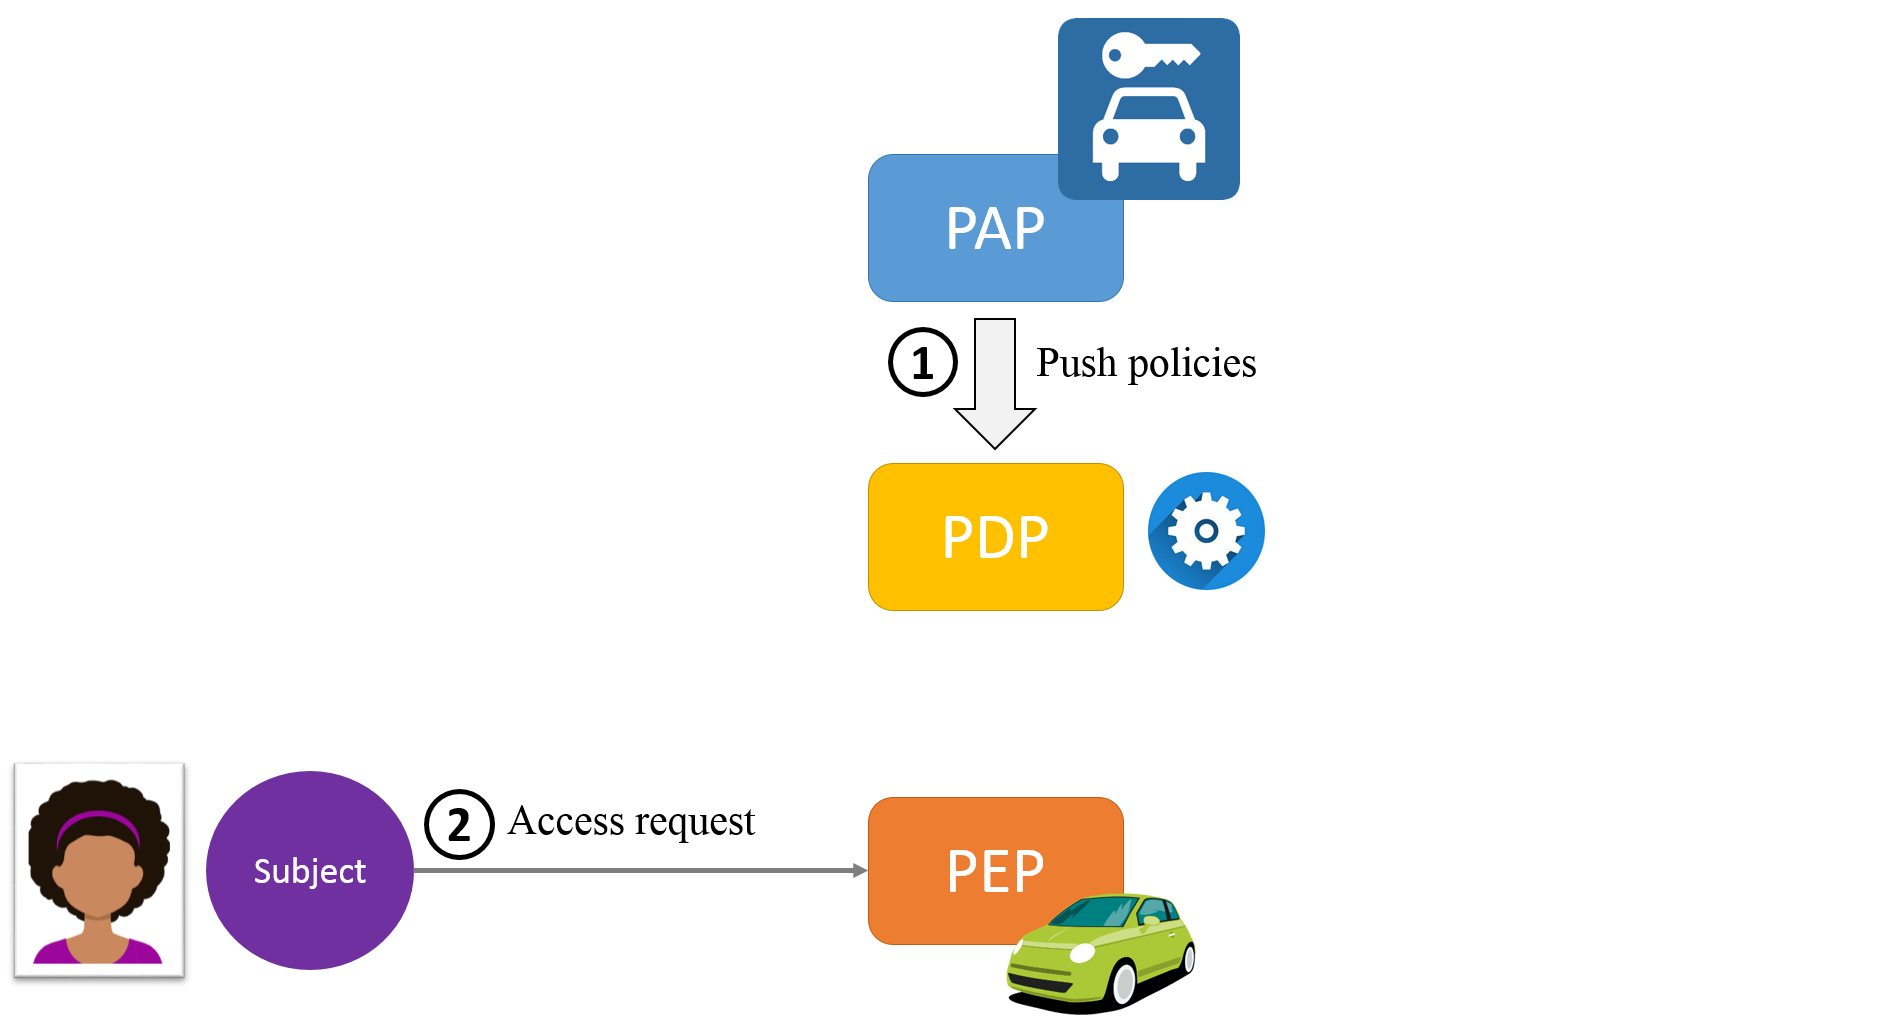
\includegraphics[scale=0.35]{Figures/AC_instance_2.png}
        \end{center}
        
        The \alert{PEP (Policy Enforcement Point~\cite{RFC2753})} is where decisions are actually enforced.
    }
        
    \only<4>{
        \begin{center}
            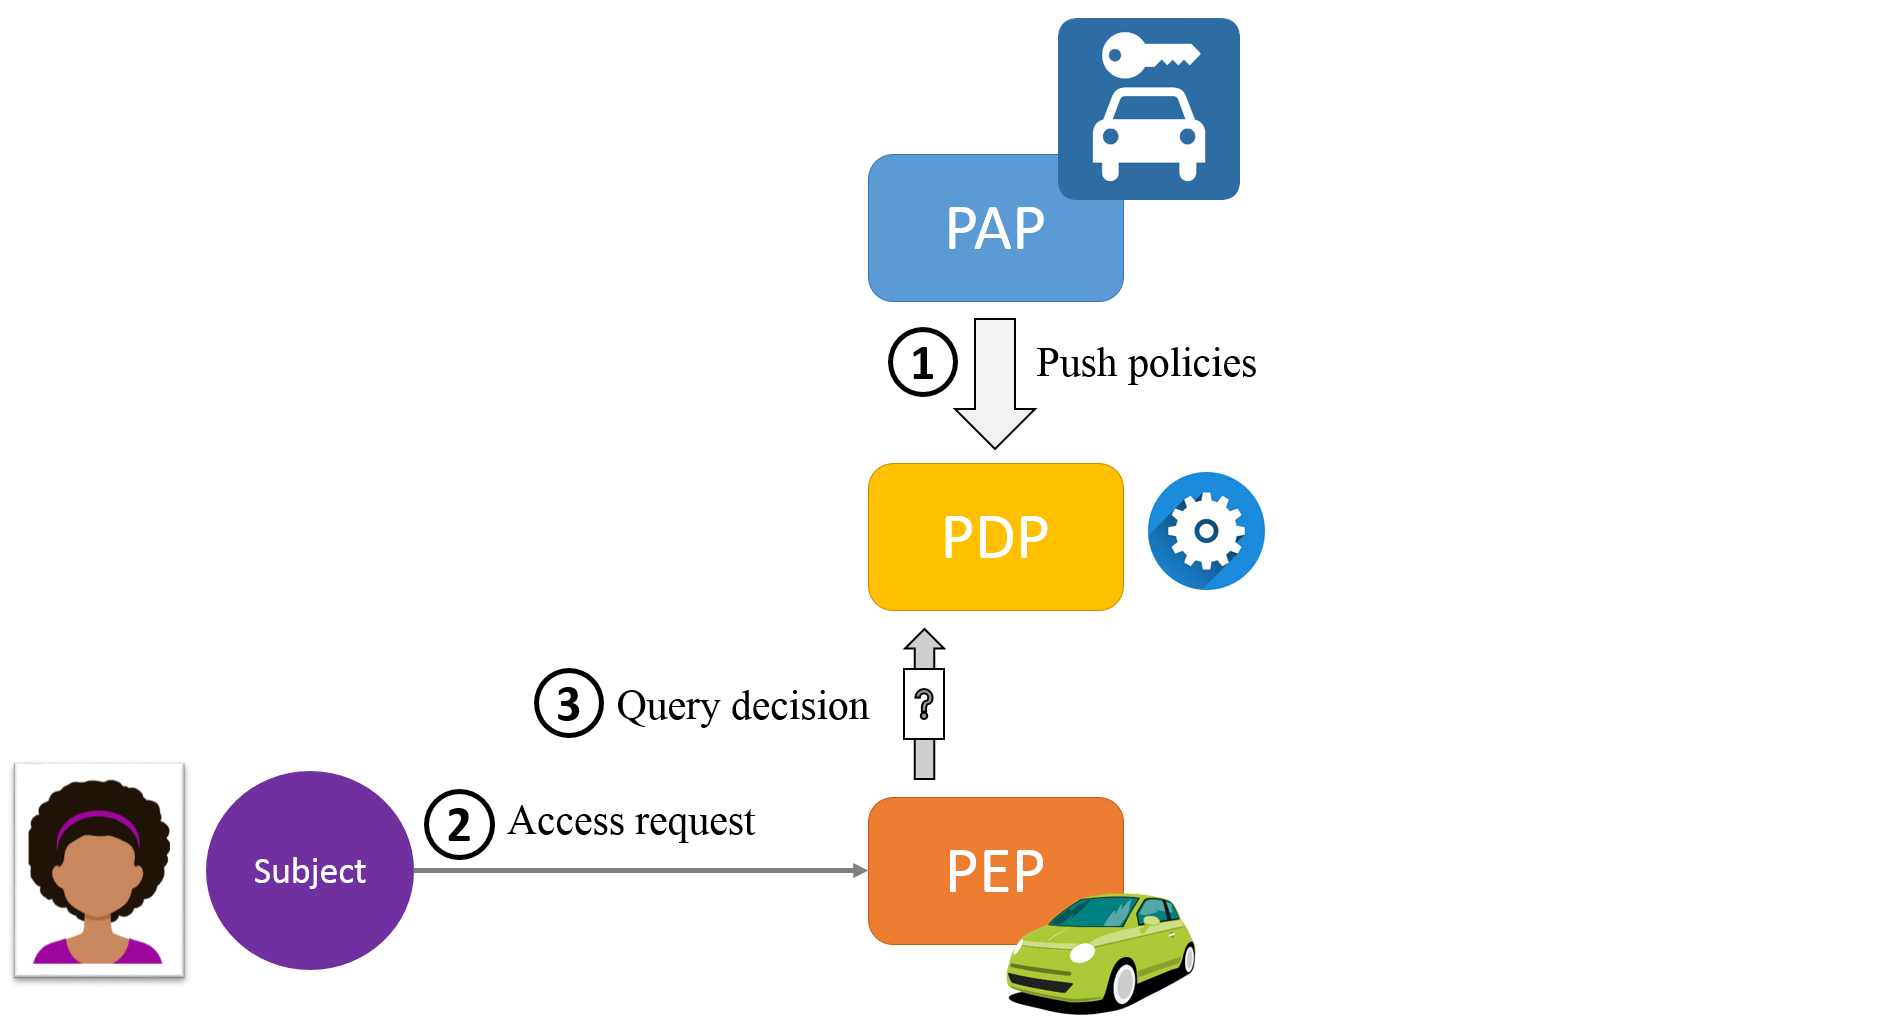
\includegraphics[scale=0.35]{Figures/AC_instance_3.png}
        \end{center}
        
        The \alert{PDP (Policy Decision Point~\cite{RFC2753})} is where decisions are made.
    }
        
    \only<5>{
        \begin{center}
            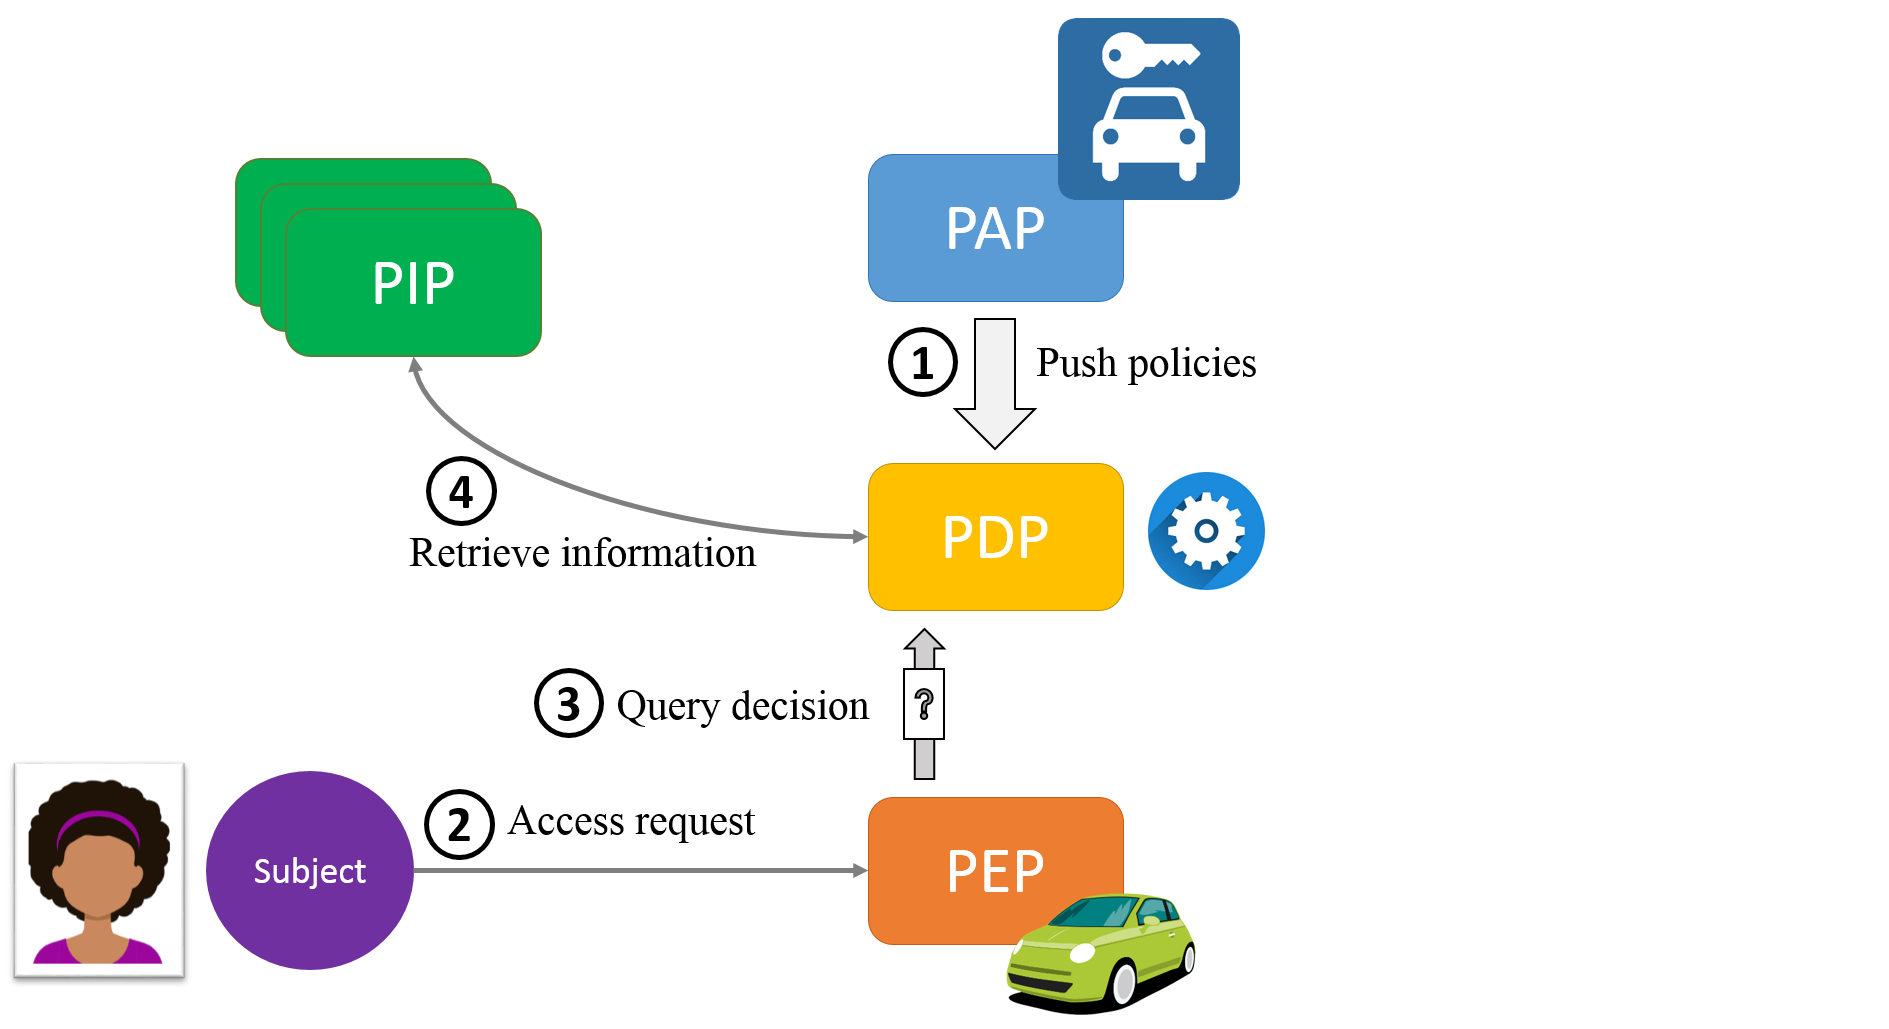
\includegraphics[scale=0.35]{Figures/AC_instance_4.png}
        \end{center}
        
        The \alert{PIP (Policy Information Point~\cite{hu2013guide})} delivers information required for the access decision.
    }
        
    \only<6>{
        \begin{center}
            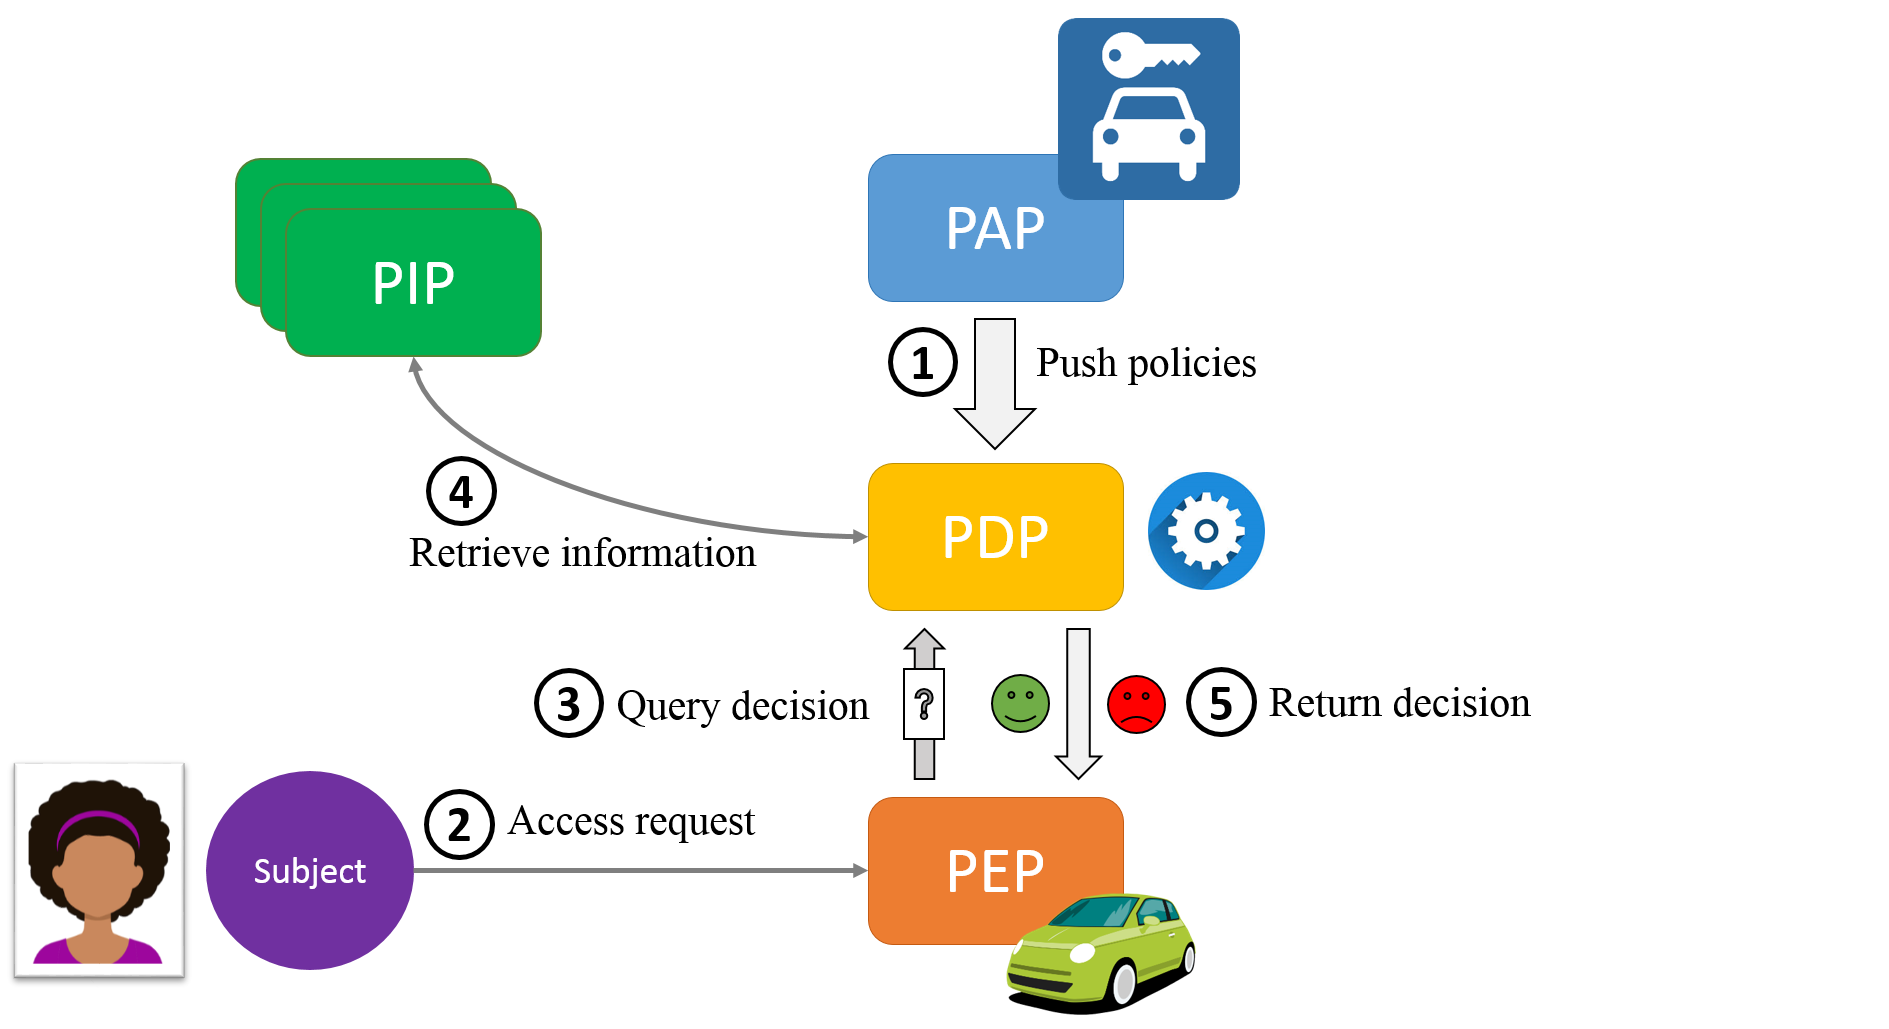
\includegraphics[scale=0.35]{Figures/AC_instance_5.png}
        \end{center}
    }
        
    \only<7>{
        \begin{center}
            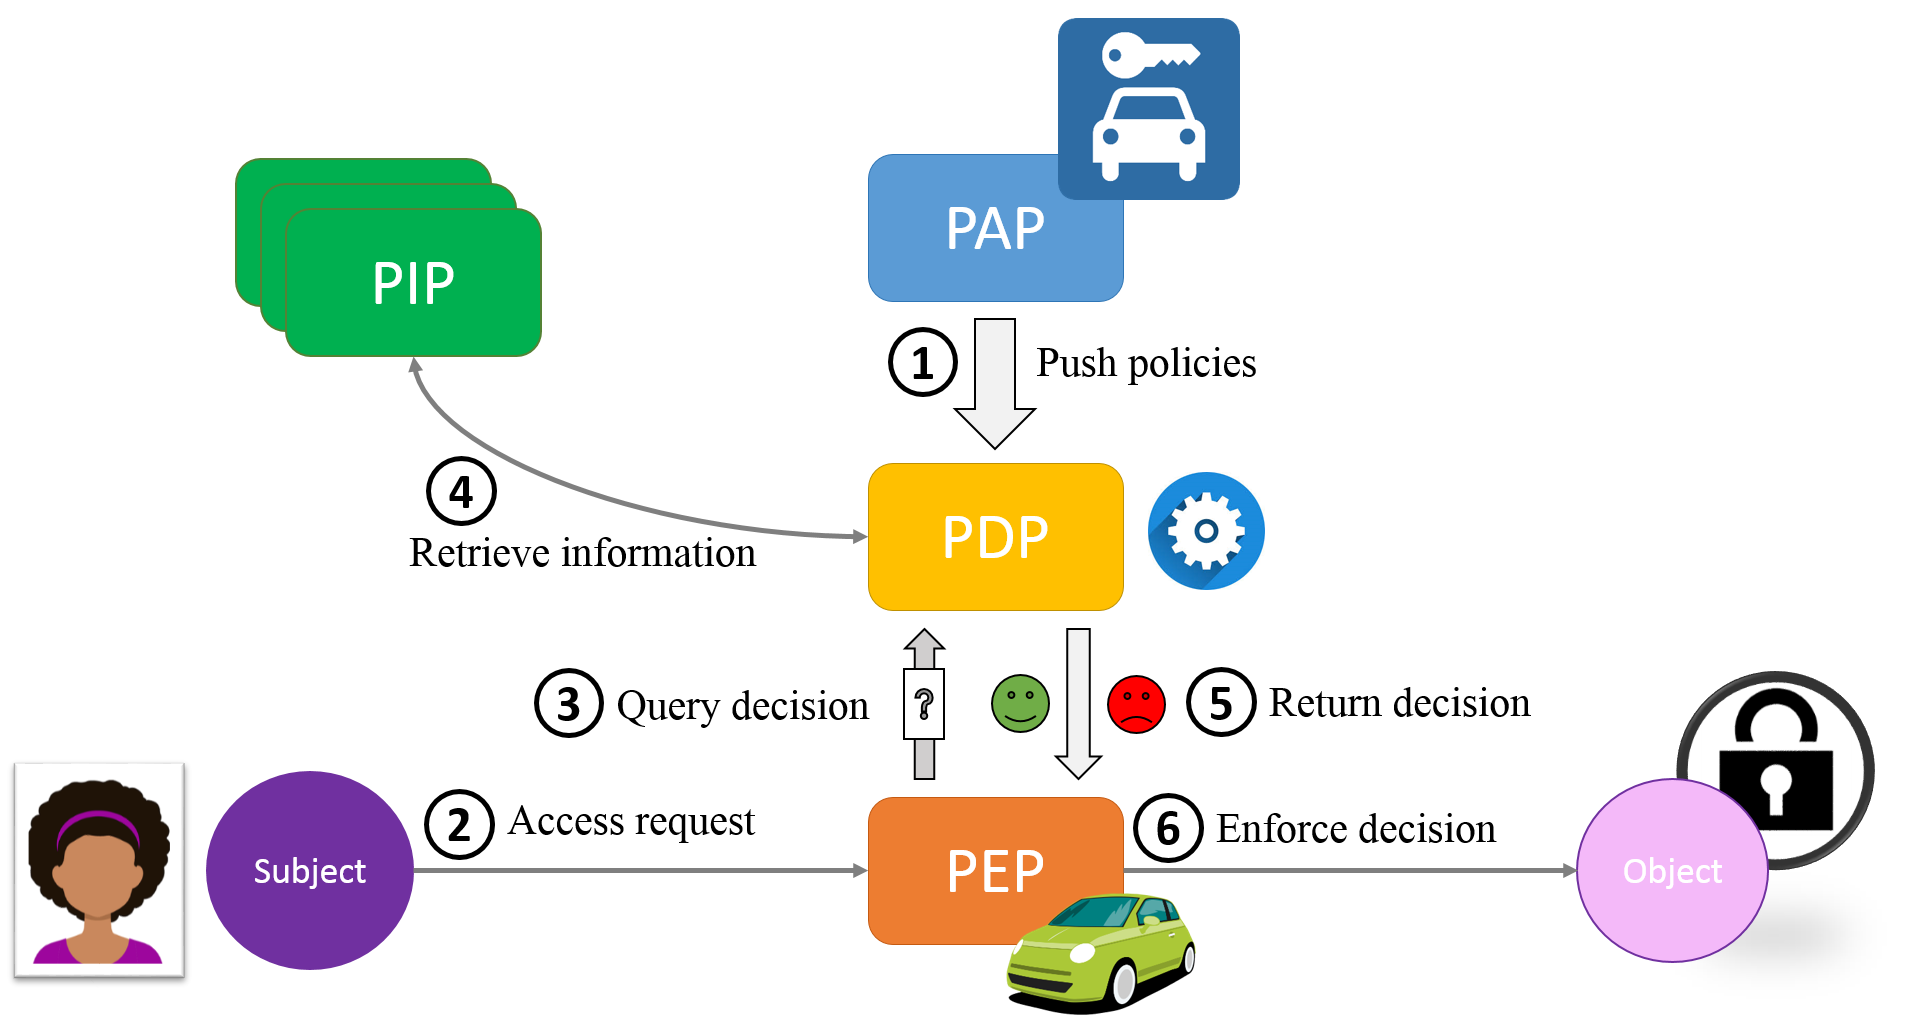
\includegraphics[scale=0.35]{Figures/AC_instance_6.png}
        \end{center}
    }
\end{frame}

% - - - - - - - - - - SUBSECTION - - - - - - - - - - %
\subsection{Access control architectures}

% * * * * * * NEW FRAME * * * * * * %
\begin{frame}{Defining architectures: Where is the PDP?}
    \begin{center}
        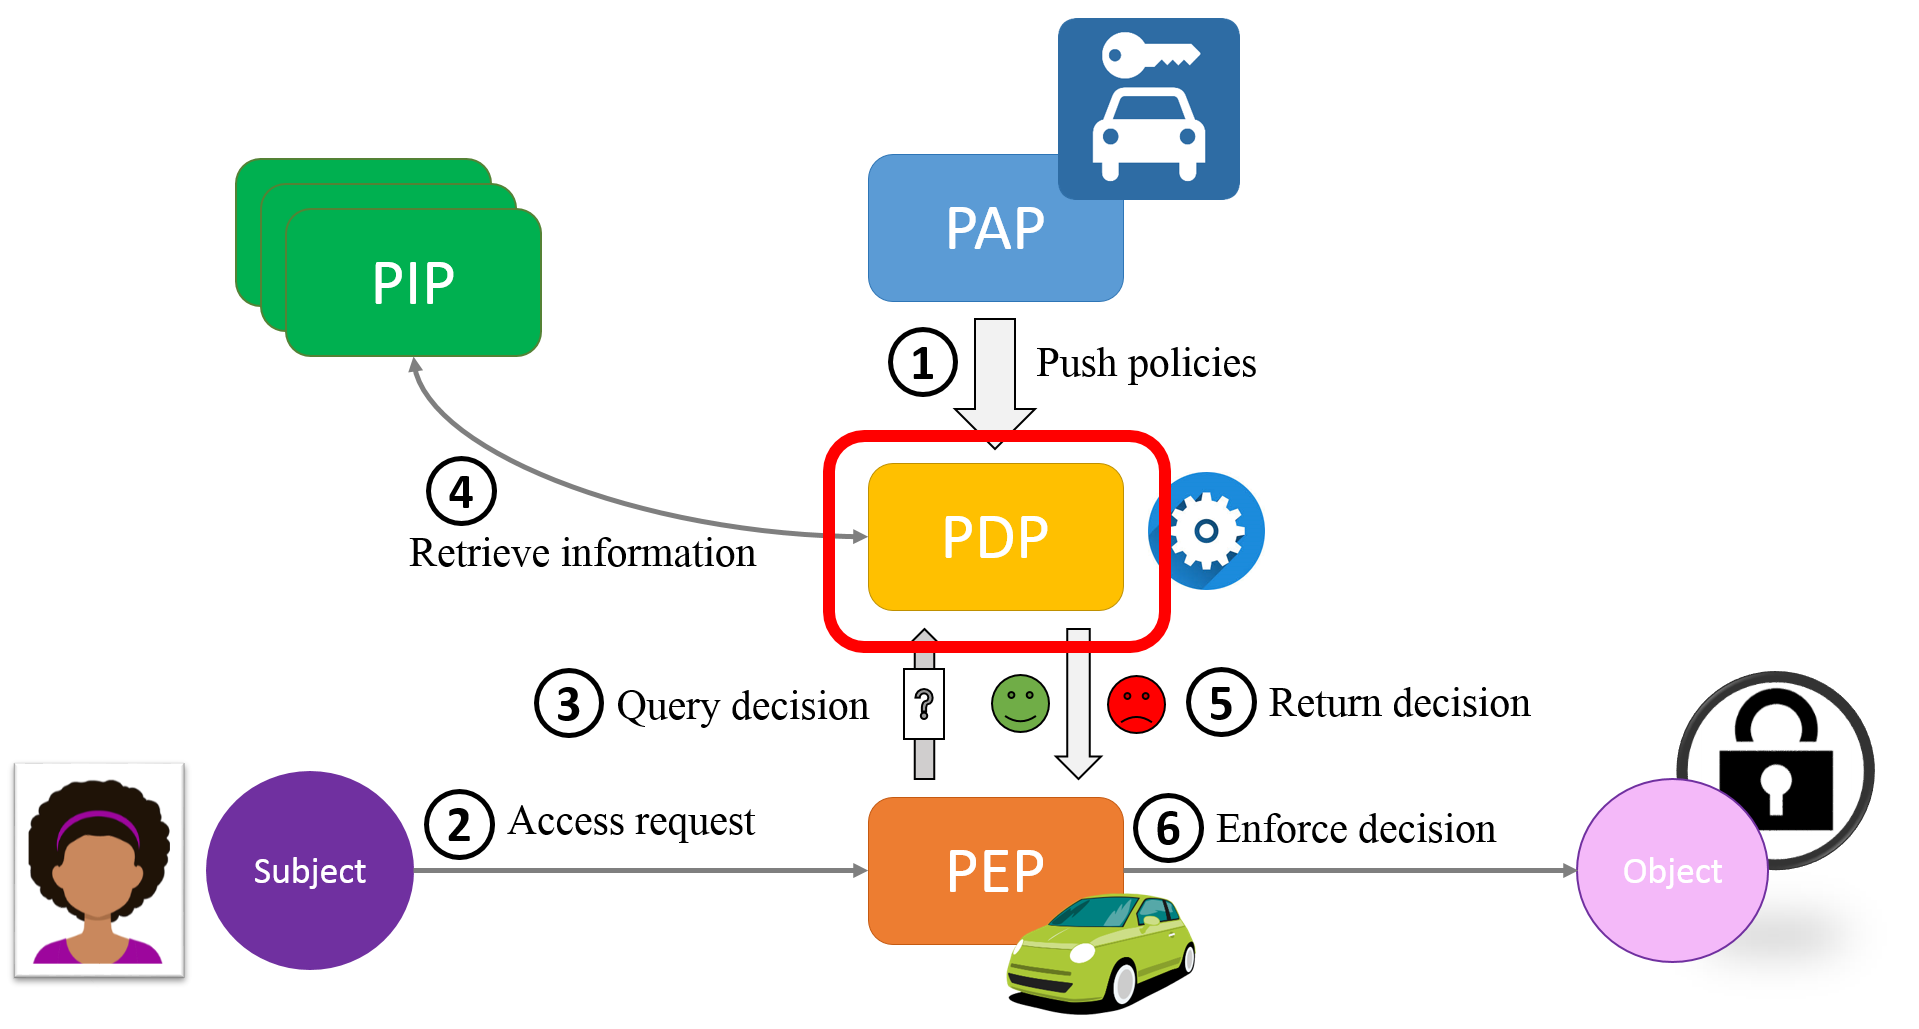
\includegraphics[scale=0.33]{Figures/AC_instance_7.png}
    \end{center}
    
\end{frame}

% * * * * * * NEW FRAME * * * * * * %
\begin{frame}{Centralized architecture: circumventing resource scarcity}
    \begin{center}
        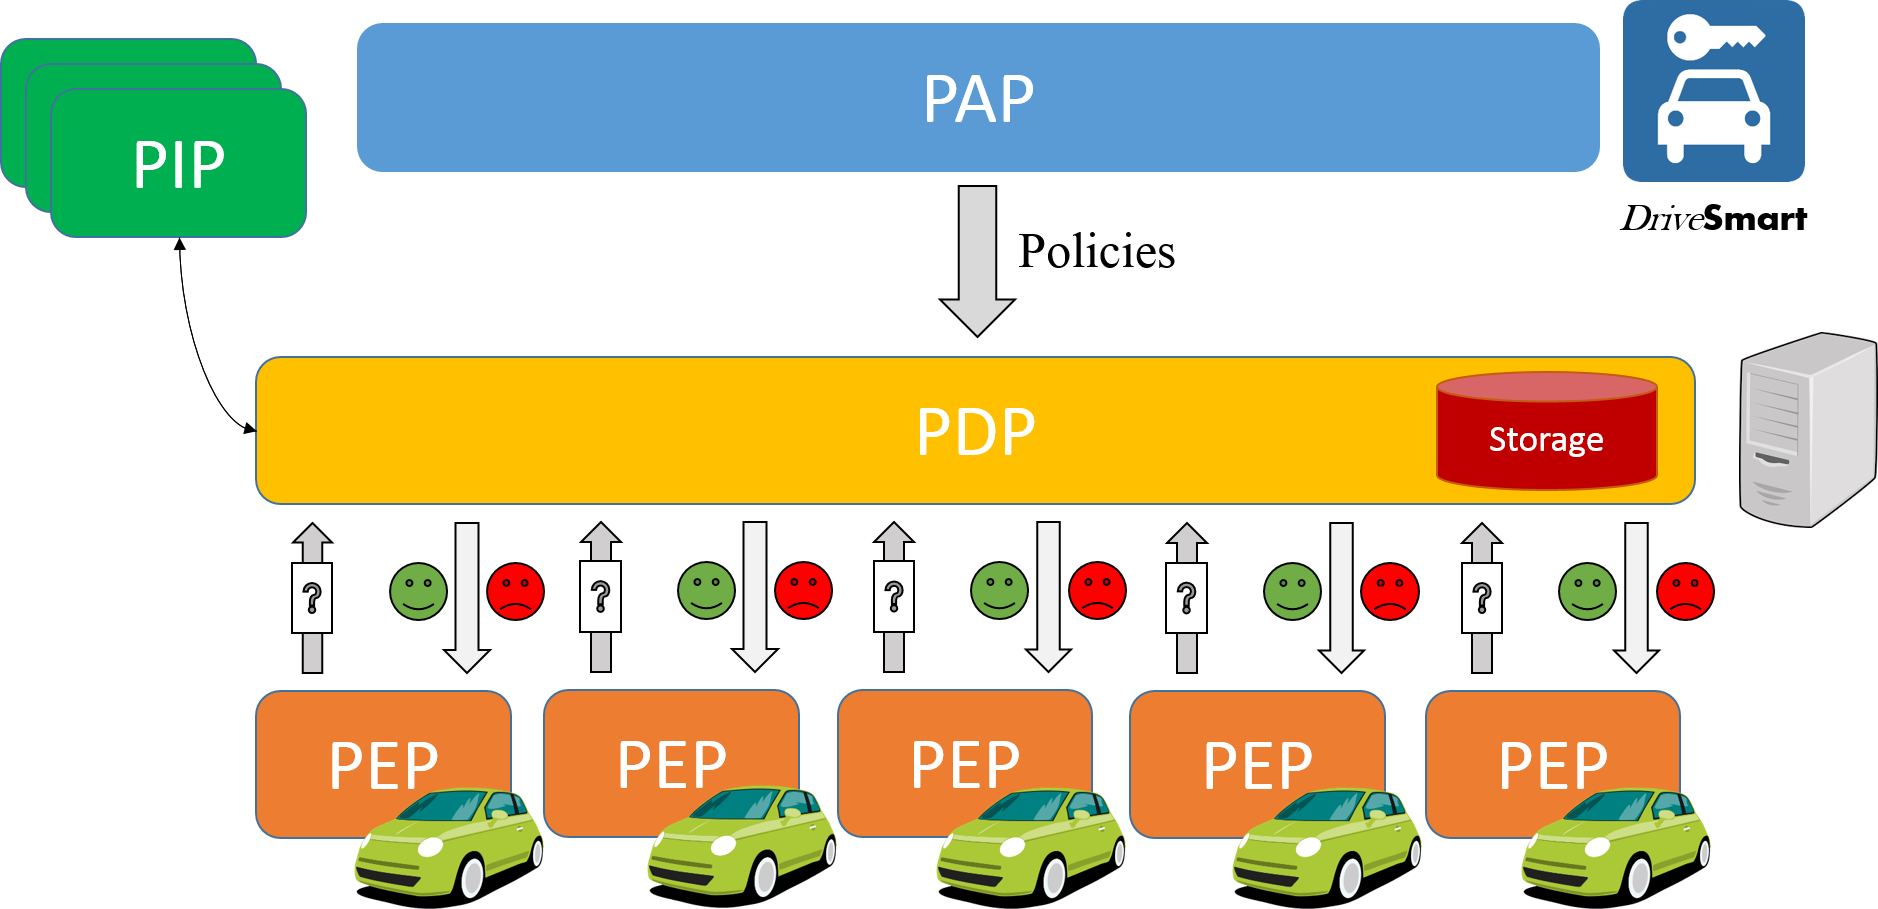
\includegraphics[scale=0.33]{Figures/central_archi.png}
    \end{center}
    
\end{frame}


% * * * * * * NEW FRAME * * * * * * %
\begin{frame}{Hierarchical architecture: Spacial or Logical separation}
    \begin{center}
        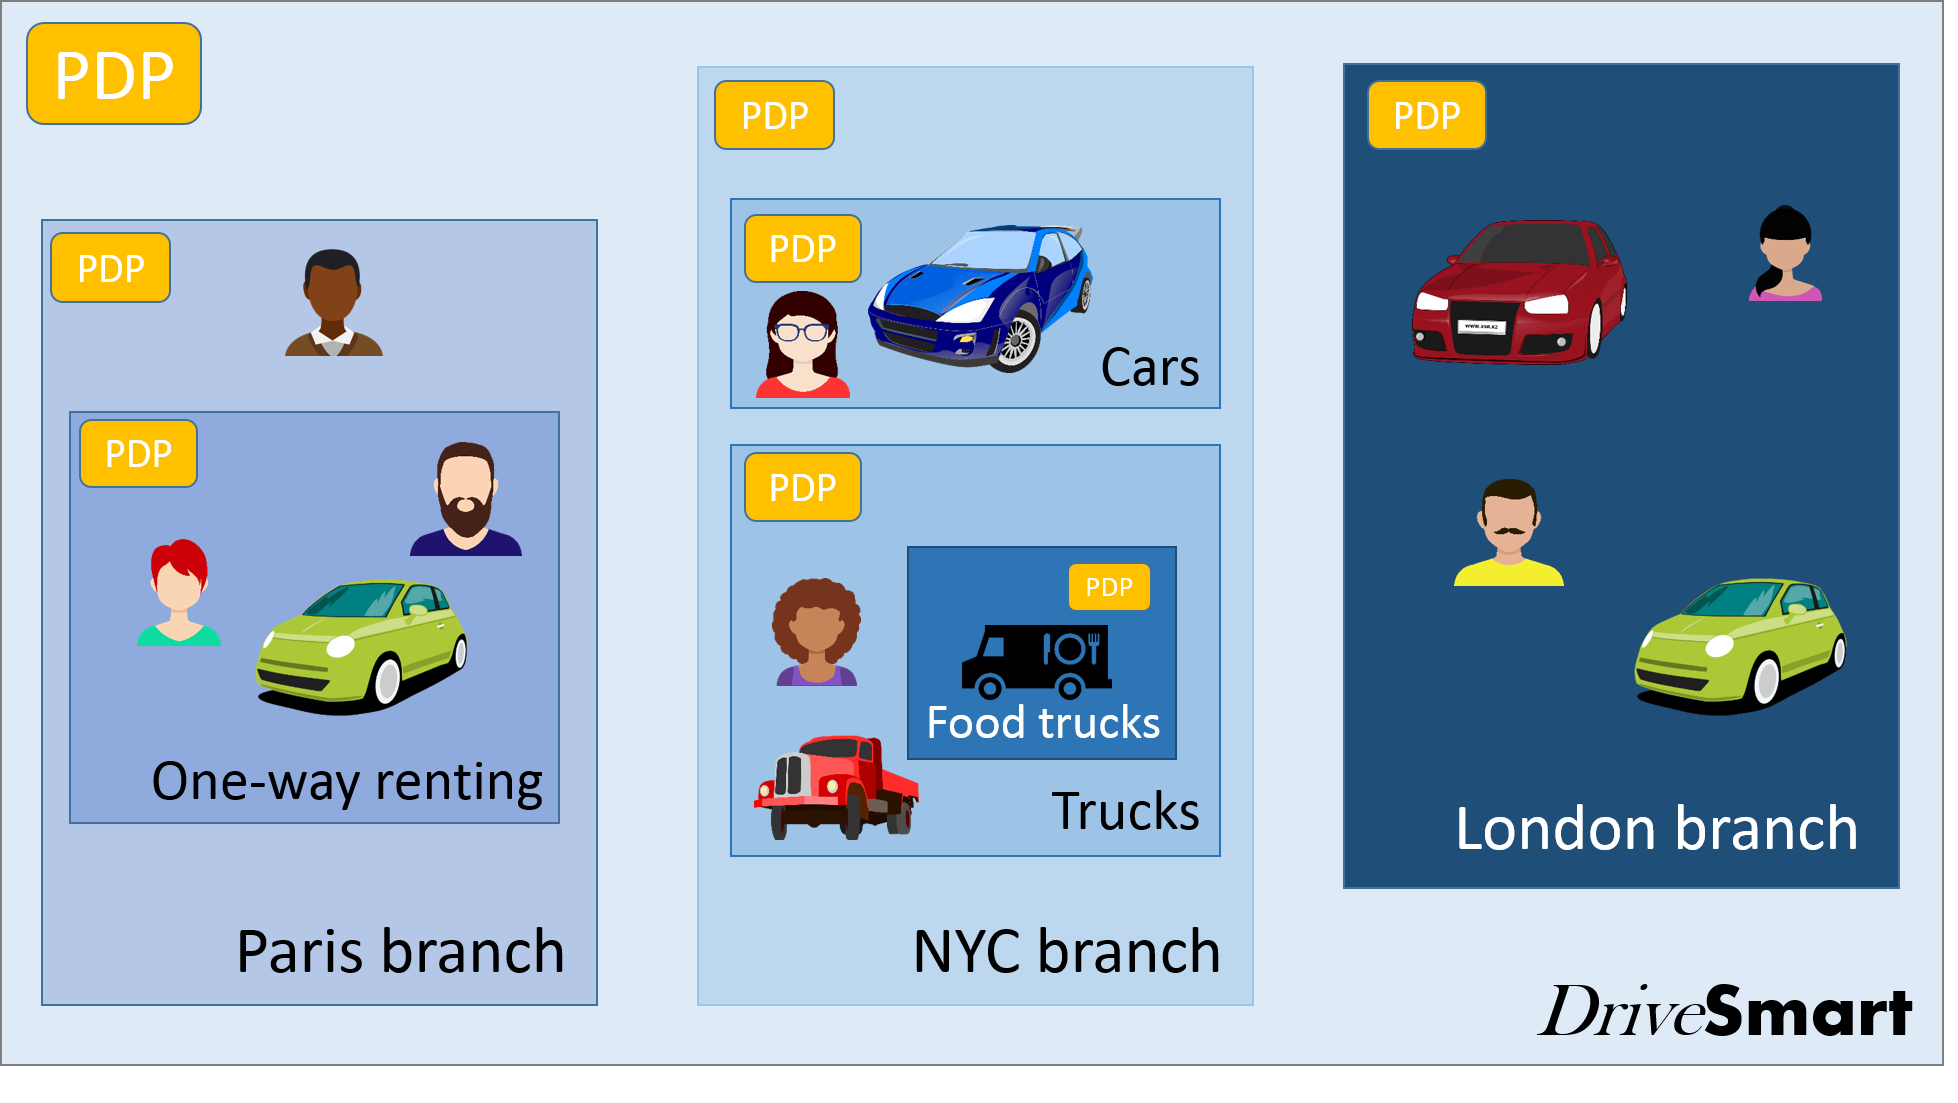
\includegraphics[scale=0.36]{Figures/hierarchical_archi_car.png}        
        \end{center}
\end{frame}


% * * * * * * NEW FRAME * * * * * * %
\begin{frame}{Federated architecture: joining security domains}
    \begin{center}
        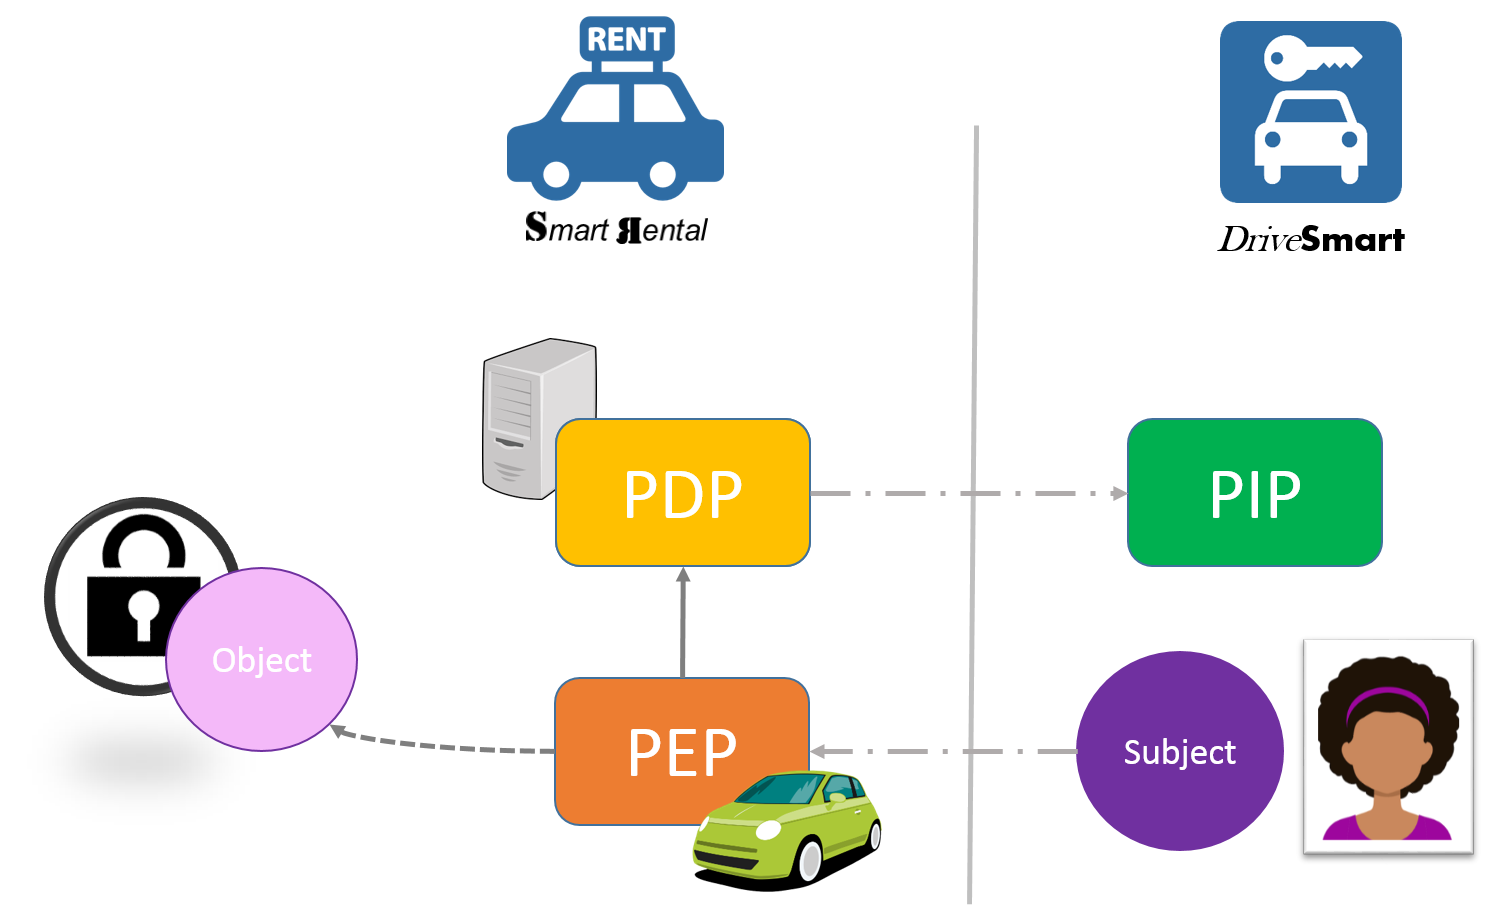
\includegraphics[scale=0.4]{Figures/federated_archi.png}
    \end{center}    
\end{frame}


% * * * * * * NEW FRAME * * * * * * %
\begin{frame}{Distributed architecture 1: Hybrid architecture}
    \begin{center}
        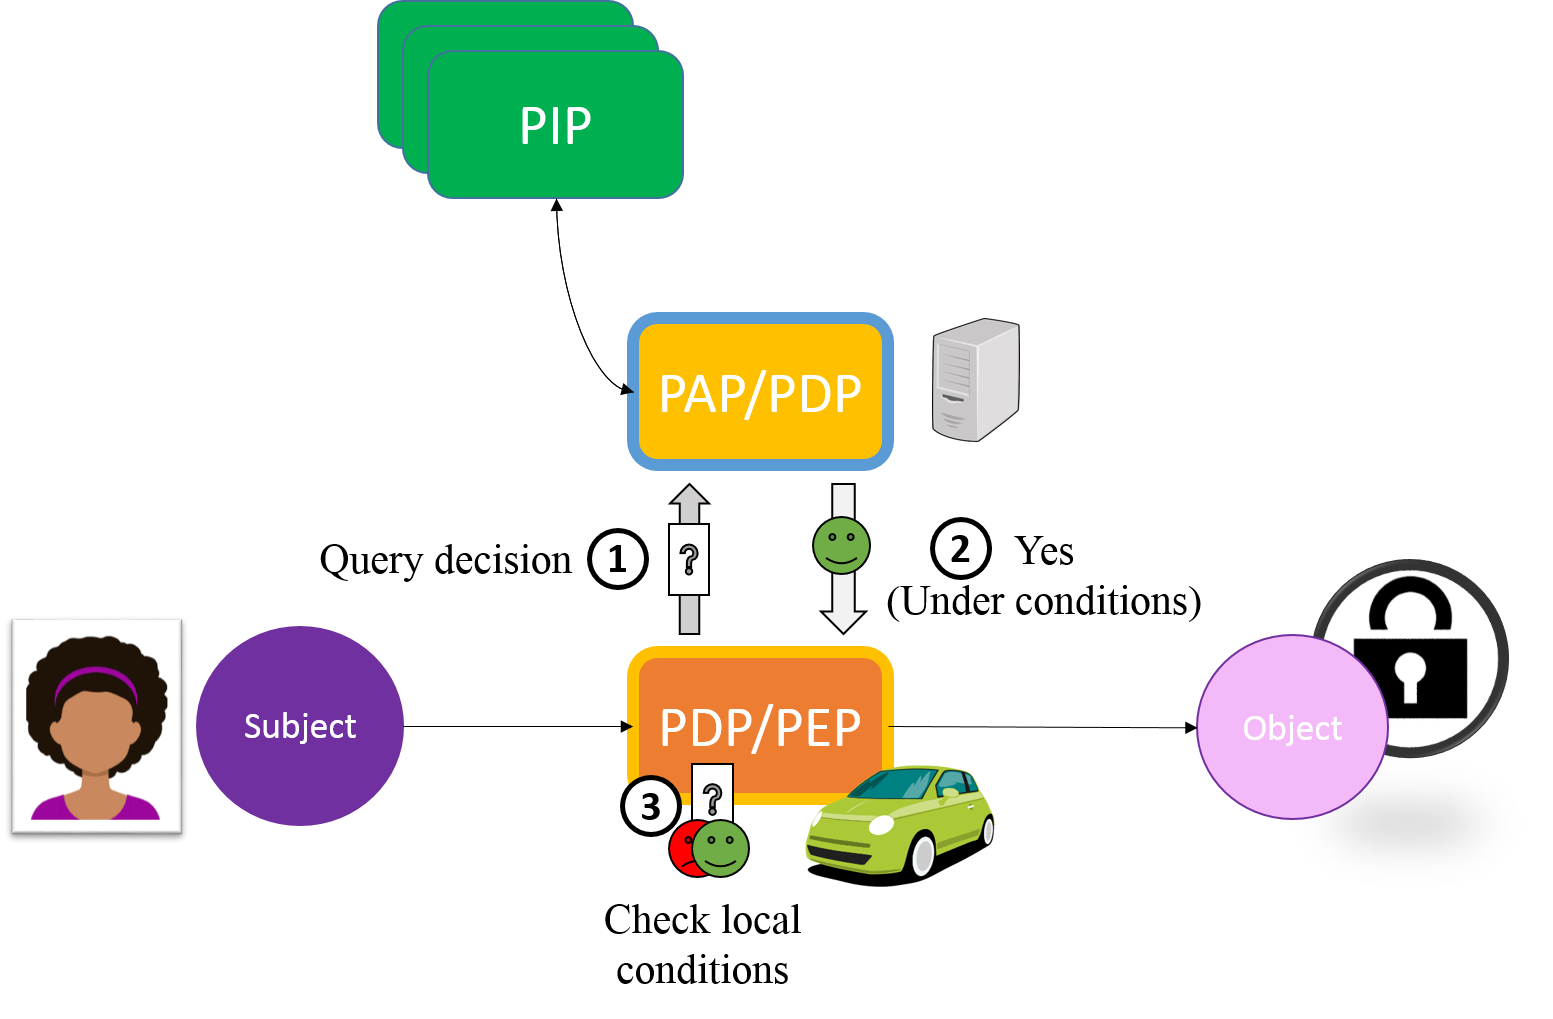
\includegraphics[scale=0.35]{Figures/hybrid_archi.png}
    \end{center}    
\end{frame}


% * * * * * * NEW FRAME * * * * * * %
\begin{frame}{Distributed architecture 2: Multi PDP architecture}
    \begin{center}
        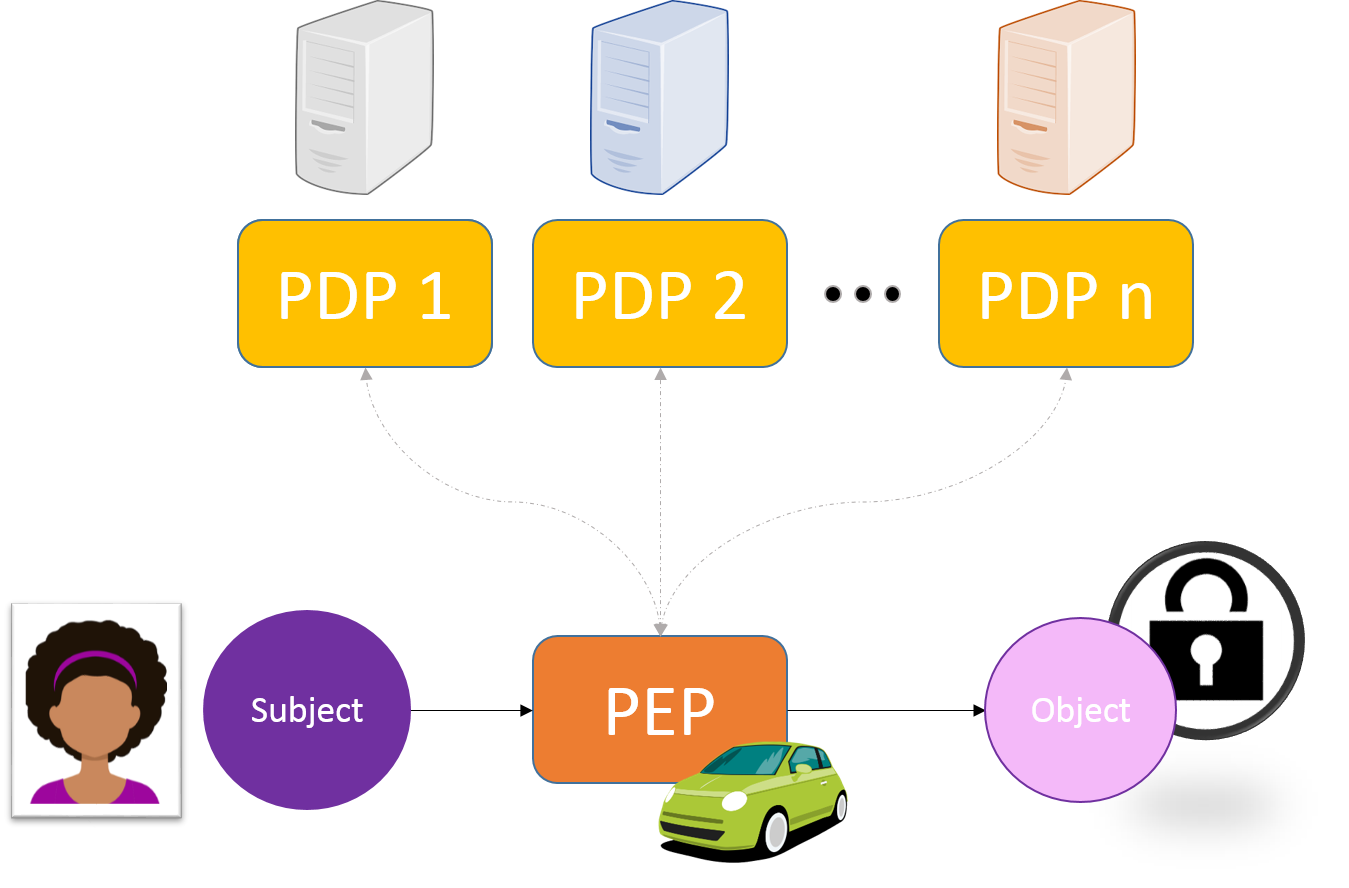
\includegraphics[scale=0.4]{Figures/multiPDP_archi.png}
    \end{center}    
\end{frame}


% * * * * * * NEW FRAME * * * * * * %
\begin{frame}{Distributed architecture 3: Blockchain-based architecture}
    \begin{center}
        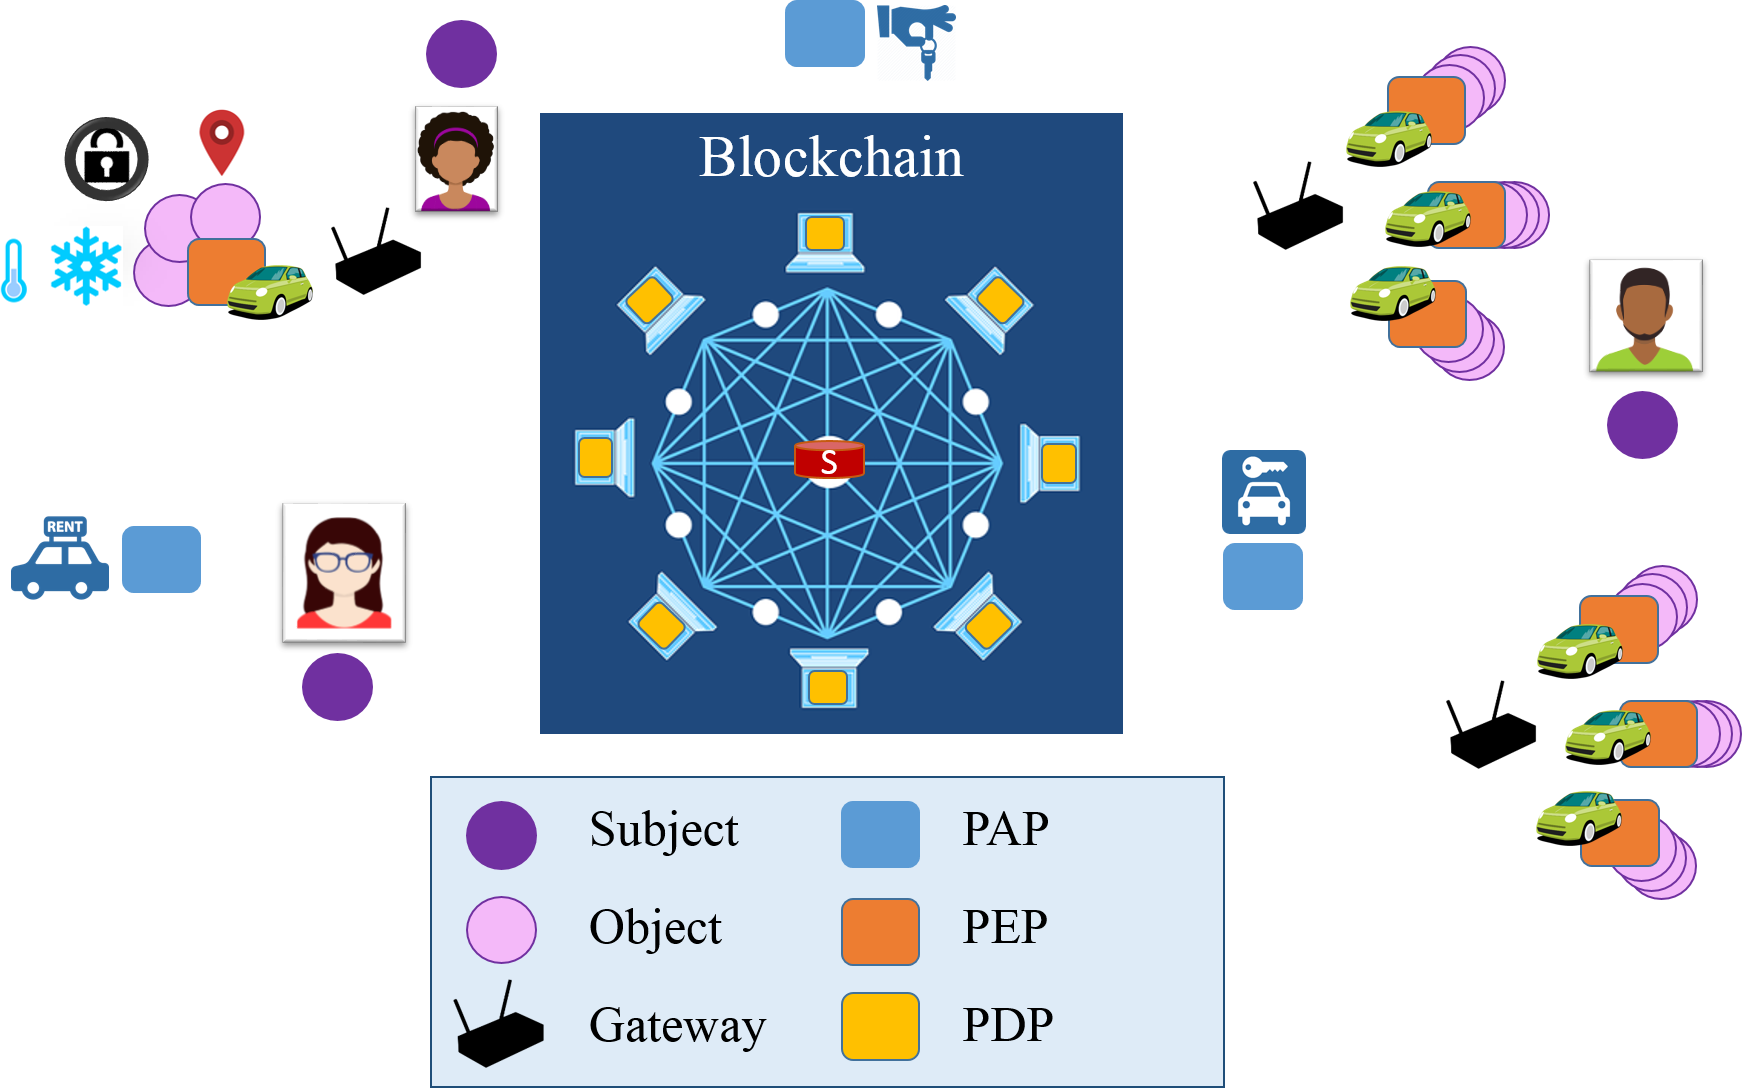
\includegraphics[scale=0.35]{Figures/bc_archi_alt.png}
    \end{center}    
\end{frame}

% - - - - - - - - - - SUBSECTION - - - - - - - - - - %
\subsection{Comparing solutions from the literature}

% * * * * * * NEW FRAME * * * * * * %
\begin{frame}{Comparison criteria}

\begin{multicols}{2}
    \begin{itemize}
        \item Registration (\textcolor{orange}{O})
        \item \highlightbox<2>{lightgray}{Resource Efficiency} (\textcolor{purple}{C})
        \item Resilience (\textcolor{purple}{C})
        \item Serverless authorization (\textcolor{orange}{O})
        \item \highlightbox<2>{lightgray}{Scalability} (\textcolor{purple}{C})
        \item Maintainability (\textcolor{purple}{C})
        \item Permission Updates (\textcolor{purple}{C})
        \item Usability (\textcolor{purple}{C})
        \item Granularity (\textcolor{orange}{O})
        \item \highlightbox<2>{lightgray}{Context-Awareness} (\textcolor{purple}{C})
        \item \highlightbox<2>{lightgray}{Revocation} (\textcolor{orange}{O})
        \item Delegation (\textcolor{orange}{O})
        \item \highlightbox<2>{lightgray}{Auditability} (\textcolor{orange}{O})
        \item Privacy (\textcolor{purple}{C})
        \item \highlightbox<2>{lightgray}{Governance} (\textcolor{orange}{O})
        \item Maturity level (\textcolor{orange}{O})
    \end{itemize}
\end{multicols}

\colorbox{lightgray}{\makebox[\textwidth-2\fboxsep][c]{\emph{\textcolor{orange}{O}: Objective
 - \textcolor{purple}{C}: Comparative}}}

\end{frame}

% * * * * * * NEW FRAME * * * * * * %
 \begin{frame}{Comparing architectures: Benefits and disadvantages}

     \begin{table}[ht!]
     \center
     {\tiny
          \begin{tabular}{ %!{\color{black}\vrule} 
          !{\onslide<1->} T{1.4cm} !{\onslide<2->} W{0.8cm} W{0.8cm} !{\onslide<3->} B{1.3cm} !{\onslide<4->} W{1.1cm} !{\onslide<5->} B{0.8cm} B{0.8cm} b !{\onslide<1->}%!{\color{black}\vrule}
          }
           \hline
          %& \multicolumn{2}{w}{Centralized} &  &  & \multicolumn{3}{b|}{Distributed}\\
           & \multicolumn{2}{w}{Centralized} &  &  & \multicolumn{3}{b}{Distributed}\\
          \multirow{-2}{*}{\textbf{Criteria}} & Serverless & Not serverless & \multirow{-2}{*}{Hierarchical}& \multirow{-2}{*}{Federated}& multi PDP & Hybrid & Blockchain \\
         	\hline
         	\hline
         %%% META CRITERIA %%%
         Resource Efficiency        & +		& \highlightbox<1>{red}{++} 	& +     & +  	& -  	& - -  &  - -   \\  \arrayrulecolor{black!30}\hline
         Resilience 				& -		& - - 	& +     & +  	& ++ 	& -    &  ++    \\  \arrayrulecolor{black!30}\hline
         Scalability 				& -		& - - 	& +     & +  	& ++ 	& -    &  +     \\  \arrayrulecolor{black!30}\hline
         Maintainability 		    & ++	& +		& -     & - -   & - -   &      &  +     \\  \arrayrulecolor{black!30}\hline
         Permission Updates 	    & - 	& ++	& +     & -  	& - -   & +    &  -     \\  \arrayrulecolor{black!30}\hline
         Usability 					& ++	& +		&       & ++ 	& -  	&      &  +     \\  \arrayrulecolor{black!30}\hline
         Context-awareness 	        & - -	& - 	& +     &    	&    	& ++   &        \\  \arrayrulecolor{black!30}\hline
         Revocation					& - -	& ++ 	& ++    & - 	& - -   &      &  +     \\  \arrayrulecolor{black!30}\hline
         Auditable 					& +		& ++ 	&       & -  	& - -   & -    &  ++    \\  \arrayrulecolor{black!30}\hline
         Privacy 					& - -   & - -	&       & ++ 	& ++ 	& +    &  -     \\  \arrayrulecolor{black!30}\hline
         Governance 				& ++	& ++ 	& +     & - -   & - -   & +    &  - -   \\  \arrayrulecolor{black!30}\hline
         	  \arrayrulecolor{black}\hline
         \end{tabular}
     }
     \end{table}
    
 \end{frame}

% * * * * * * NEW FRAME * * * * * * %
\begin{frame}{Taxonomy}
        \begin{center}
            \only<1>{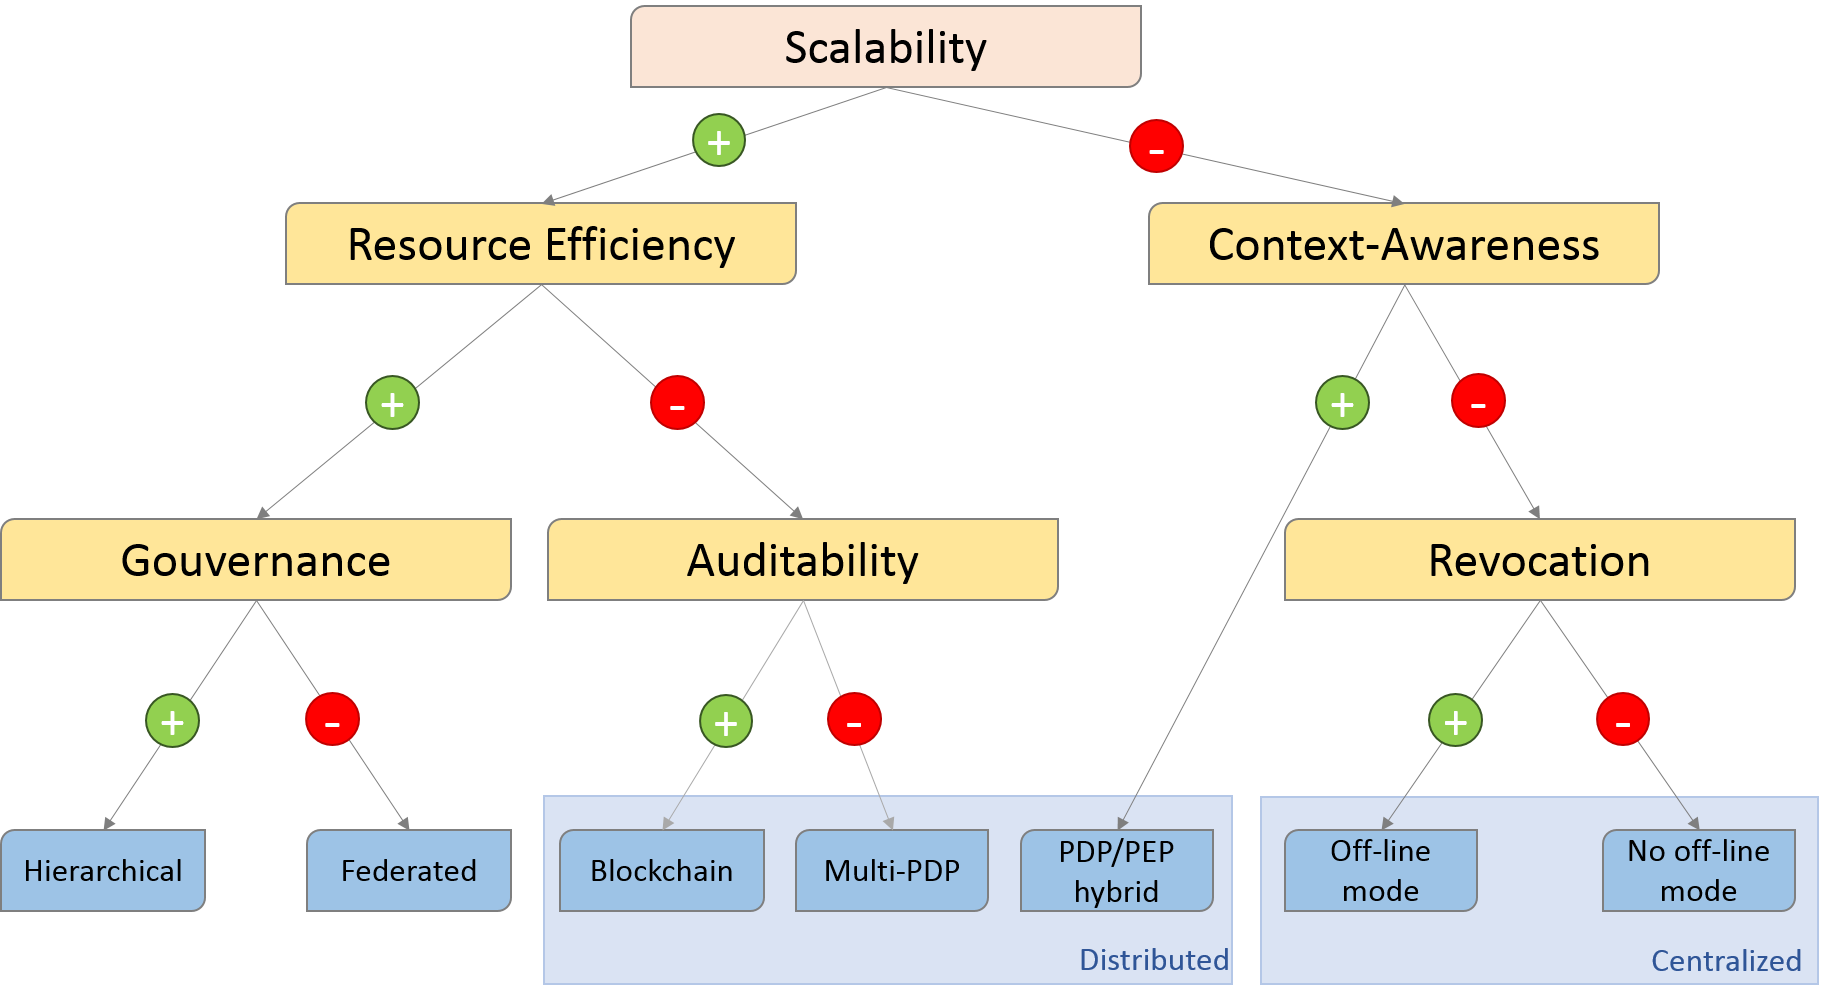
\includegraphics[scale=0.37]{Figures/taxo.png}}
            \only<2>{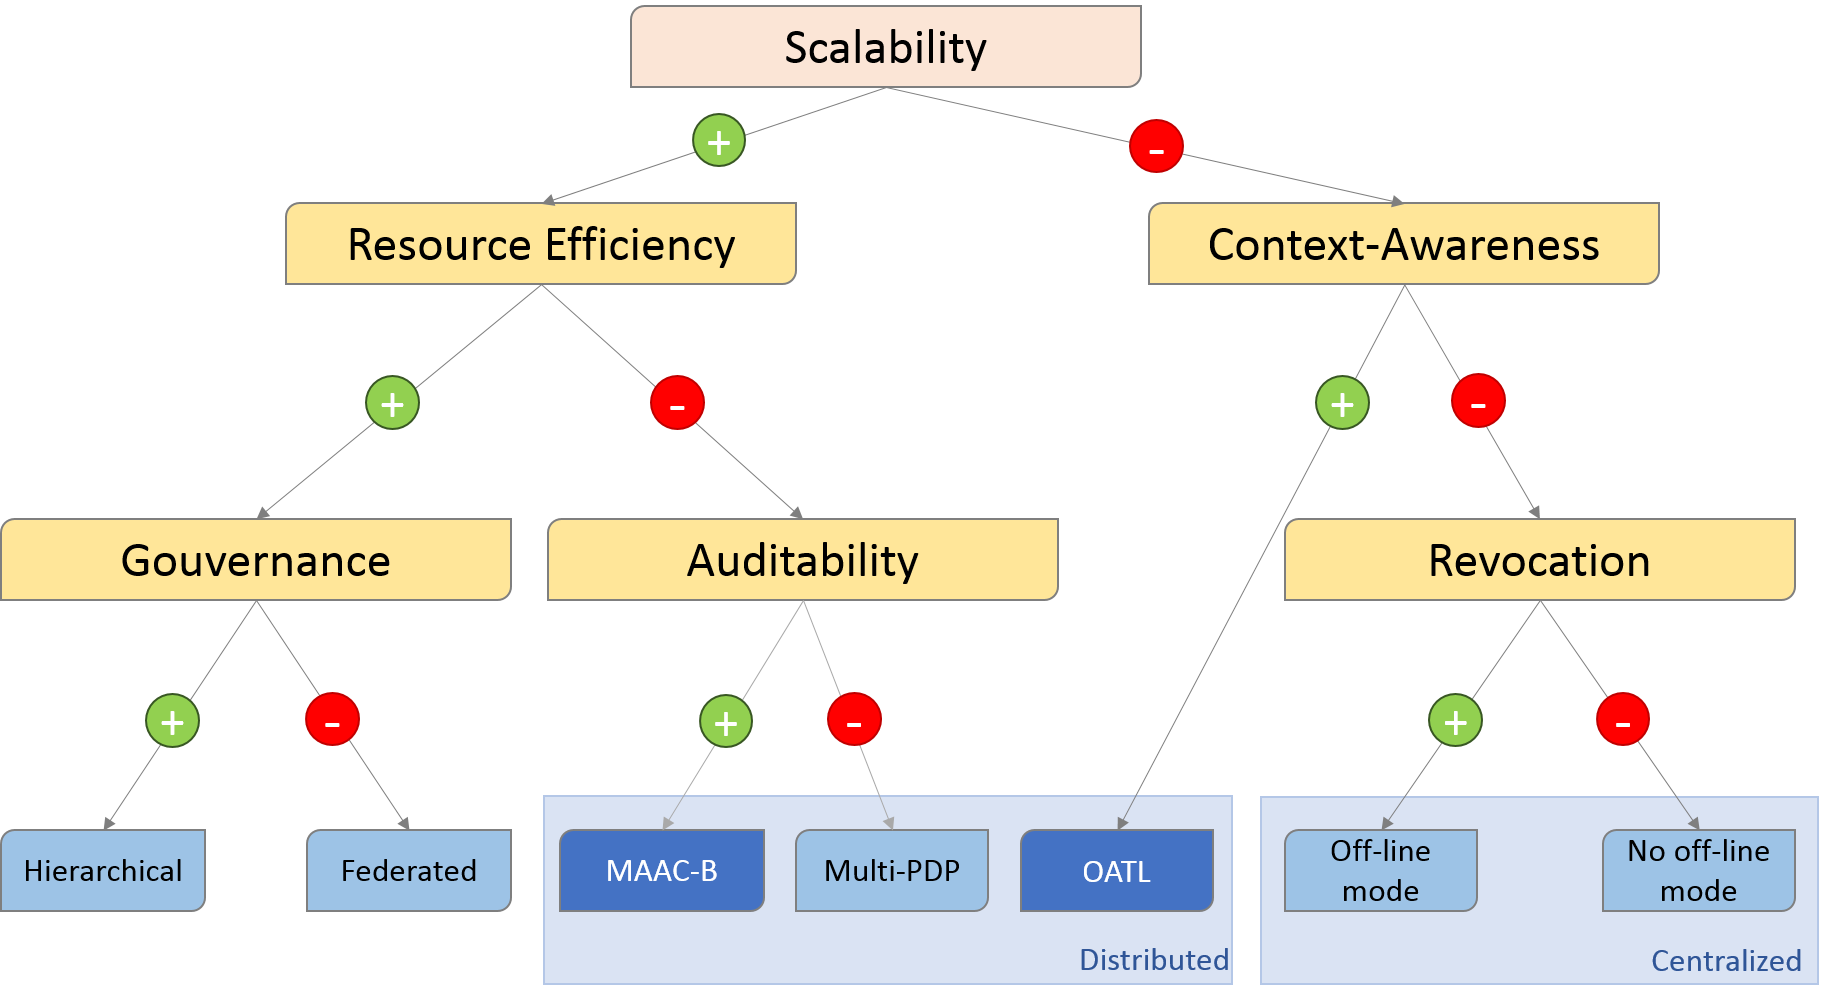
\includegraphics[scale=0.37]{Figures/taxo_2.png}}
        \end{center}
\end{frame}


% - - - - - - - - - - SUBSECTION - - - - - - - - - - %
\subsection{Conclusion}



% * * * * * * NEW FRAME * * * * * * %
\begin{frame}{Our goals}
    \begin{itemize}
        \item[$\rightarrow$] Reduce dependence to a central server
        \begin{itemize}
            \item Serverless authorization
            \item Blockchain-based system
        \end{itemize}
        \item[$\rightarrow$] Increase usability
        \begin{itemize}
            \item for users
            \item for vendors
            \item for administrators
        \end{itemize}
        \item[$\rightarrow$] Offer flexibility
        \begin{itemize}
            \item accept dynamic users
            \item accommodate changes in organizations
            \item adapt to different use cases
        \end{itemize}
        % \item[$\rightarrow$] Blockchain-based system
        
        
    \end{itemize}
\end{frame}

% * * * * * * NEW FRAME * * * * * * %
\begin{frame}{Outline}
    \begin{center}
        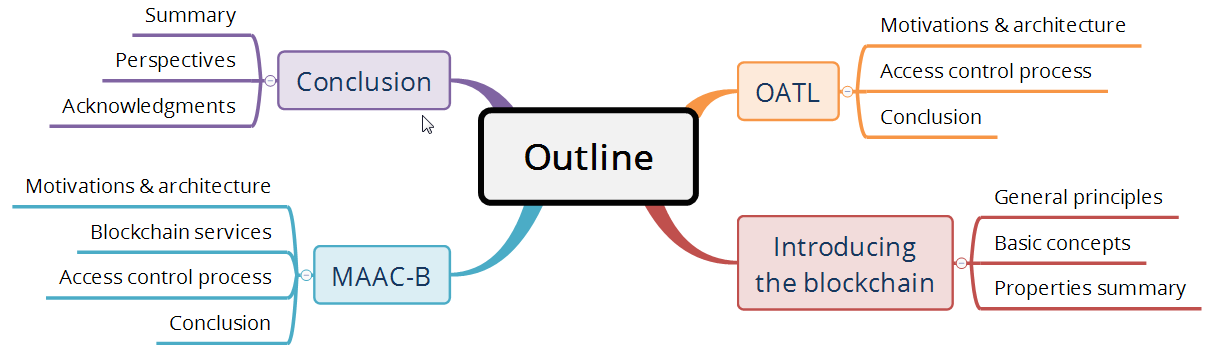
\includegraphics[scale=0.47]{Figures/Outline.png}
    \end{center}
\end{frame}
